% RLJ main.tex Version 2026.1, stubbed for the good-regulator RLC 2027 submission.
% Page limit: 8--12 pages of main text. Appendices BEFORE the references count toward it;
% material after \beginSupplementaryMaterials does not, and must hold nothing central.

\documentclass[10pt]{article}

% \usepackage{rlj}           % submission (anonymous)
%\usepackage[accepted]{rlj} % camera-ready
\usepackage[preprint]{rlj} % de-anonymised preprint

\usepackage{amssymb}
\usepackage{mathtools}
\usepackage{mathrsfs}
\usepackage{graphicx}
\usepackage{subcaption}
\usepackage[space]{grffile}
\usepackage{url}
\usepackage{amsthm}
\usepackage{booktabs}
\usepackage{tikz}
\usetikzlibrary{positioning,fit,arrows.meta,decorations.pathreplacing,calc,shapes.geometric}
% Empty axes for a result panel not yet produced. Usage: \stubplot{x label}{y label}
\newcommand{\stubplot}[2]{%
  \begin{tikzpicture}
    \draw[->] (0,0) -- (4.6,0) node[below left, font=\scriptsize] {#1};
    \draw[->] (0,0) -- (0,2.8) node[above right, font=\scriptsize] {#2};
    \draw[dashed, gray] (0.15,0.15) rectangle (4.4,2.55);
    \node[gray, font=\scriptsize\itshape] at (2.3,1.35) {placeholder};
  \end{tikzpicture}%
}
 % figure stubs, remove before submission

\graphicspath{{figs/}}

%%%%%%%%%%%%%%%%%%%%%%%%%%%%%%%%%%%%%%%%%%%%%%%%%%%%%%%%%%%%%%%%
% Notation, following notes_joery/theory_to_algorithm_joery_v2.tex
%%%%%%%%%%%%%%%%%%%%%%%%%%%%%%%%%%%%%%%%%%%%%%%%%%%%%%%%%%%%%%%%
\newcommand{\Scal}{\mathcal S}
\newcommand{\Acal}{\mathcal A}
\newcommand{\Zcal}{\mathcal Z}
\providecommand{\Lcal}{\mathcal L}
\newcommand{\Dcal}{\mathcal D}
\newcommand{\E}{\mathbb E}
\newcommand{\occ}{d^{\pi}}
\newcommand{\Occ}{\mathscr D}   % occupancy polytope; \Dcal is the disturbance alphabet
\newcommand{\pz}{p_{\pi}}
\newcommand{\Hnu}[1]{H_{\nu}\!\left[#1\right]}
\newcommand{\KL}{\mathrm{KL}}
\newcommand{\dd}{\mathrm d}

\theoremstyle{plain}
\newtheorem{theorem}{Theorem}
\newtheorem{proposition}{Proposition}
\newtheorem{lemma}{Lemma}
\newtheorem{corollary}{Corollary}
\theoremstyle{definition}
\newtheorem{definition}{Definition}

% Tracked edits. \add = red insertion, \del = red strikethrough. Remove before submission.
\usepackage[normalem]{ulem}
\newcommand{\add}[1]{\textcolor{red}{#1}}
\newcommand{\del}[1]{\textcolor{red}{\sout{#1}}}

% Planning macros. Remove before submission: grep for \todo and \intent.
\newcommand{\todo}[1]{\textcolor{red!70!black}{[TODO: #1]}}
\newcommand{\intent}[1]{\par\noindent\textcolor{blue!60!black}{\small\textit{Intent: #1}}\par}
\newcommand{\budget}[1]{\textcolor{gray}{\small[budget: #1]}}



% Working title; the overall frame is not decided yet. write down more ideas
\title{Good Regulators make Predictable Policies}

\setrunningtitle{Good Regulators make Predictable Policies}

\author{Joery A. de Vries\textsuperscript{1}, Neil D. Lawrence\textsuperscript{1,2}}

\emails{\{joery,neil\}@trent.ai, ndl21@cam.ac.uk}

\affiliations{
$^{1}$\textbf{Trent AI Limited, London, United Kingdom}\\
$^{2}$\textbf{Computer Laboratory, University of Cambridge, Cambridge, United Kingdom}
}

\contribution{
    We state Conant and Ashby's good regulator as a reinforcement-learning objective, the entropy $\min_\pi H_\nu(Z)$ of the event law over the occupancy, and show that variance MDPs, homeostatic RL and surprise minimisation are special cases or relaxations of it.
    }
    {
    The criterion is stated as ergodic sensory entropy by \citet{Friston-free12c} and minimised open loop by \citet{Adurthi-minimum14}.
    The deterministic optimum follows from the concave-occupancy results of \citet{Derman-finite70ch7} and \citet{Piunovskiy-controlled98}, and the variance line has it already \citep{Filar-variance89,Sobel-meanvariance94}.
    }

\keywords{good regulator, homeostasis, convex reinforcement learning}

\summary{
We develop a reinforcement learning (RL) recipe framed around the good regulator from cybernetics.
It reuses the machinery from convex RL to minimize the entropy of an outcome law represented by the pushforward of an agent's state-action occupancy measure.
Our recipe seeks policies that are predictable, averse to uncontrollable effects and noise, and provides a necessary modelling condition of the environment to reduce said entropy.
At face value, our formulation suffers from the dark room problem, where the agent seeks a trivial but stable solution.
We therefore derive a goal-seeking condition and enable identifiability through a necessary floor on the mutual information of our agent's model to the outcome law.
On simple reward-free, deep-exploration, and continuous control tasks we confirm the efficacy and generality of our framework.
}

%%%%%%%%%%%%%%%%%%%%%%%%%%%%%%%%%%%%%%%%%%%%%%%%%%%%%%%%%%%%%%%%
\begin{document}

\makeCover
\maketitle

% One paragraph of 4-6 sentences, written last.
\begin{abstract}
We develop a reinforcement learning (RL) recipe framed around the good regulator from cybernetics.
It reuses the machinery from convex RL to minimize the entropy of an outcome law represented by the pushforward of an agent's state-action occupancy measure.
Our recipe seeks policies that are predictable, averse to uncontrollable effects and noise, and provides a necessary modelling condition of the environment to reduce said entropy.
At face value, our formulation suffers from the dark room problem, where the agent seeks a trivial but stable solution.
We therefore derive a goal-seeking condition and enable identifiability through a necessary floor on the mutual information of our agent's model to the outcome law.
On simple reward-free, deep-exploration, and continuous control tasks we confirm the efficacy and generality of our framework.
\end{abstract}

%%%%%%%%%%%%%%%%%%%%%%%%%%%%%%%%%%%%%%%%%%%%%%%%%%%%%%%%%%%%%%%%
% !TEX root = ../main.tex
%%%%%%%%%%%%%%%%%%%%%%%%%%%%%%%%%%%%%%%%%%%%%%%%%%%%%%%%%%%%%%%%
\section[Introduction]{Introduction}\label{sec:intro}

Autonomous agents are increasingly deployed in the world, from software agents acting in cyberspace \citep{Jimenez-swebench24,Yang-sweagent24,Zhang-cybench25} to robots and self-driving cars \citep{Kober-reinforcement13,Kiran-deep22}.
Reinforcement learning (RL) is a key ingredient for such agents, yet efficient and reliable algorithms remain an open problem.
Every algorithm abstracts the world through assumptions, such as a Markov state, a given reward or a stationary environment, yet real systems tend to break several of these assumptions simultaneously \citep{Dulac-Arnold-challenges21}.
So far, most of RL builds on the dynamic programming foundation of \citet{Bellman-dynamic57} or on policy gradients \citep{Williams-simple92,Sutton-policy00}, and each broken assumption has met extensions that increase algorithm complexity to counter that of the world.
As RL scales up to the real world, this complexity compounds and it becomes increasingly important to revisit ideas and ask which recipes give effective but also more manageable solutions for when assumptions break.


The good regulator of \citet{Conant-good70} is an alternative recipe from cybernetics that frames control as both an objective and a modelling problem.
A regulator acts on a system so as to leave minimal entropy in an outcome law, and the simplest regulator that achieves this must be a model of that system.
The criterion thus asks for the coarsest map $\pi$ from states to actions that minimises this entropy.
An overly abstract model merges states the outcome depends on and leaves residual entropy, while one that is too granular doesn't lower entropy but at worst spreads the outcome law.


Convex RL \citep{Zahavy-reward21,Mutti-convex23} provides a unifying language to formulate such criteria as losses on the occupancy $\occ \in \Delta(\Scal \times \Acal)$, which is the long-run distribution over states $s \in \mathcal S$ and actions $a \in \mathcal A$ as an agent's policy $\pi: \mathcal S \rightarrow \mathcal A$ is deployed in a Markov decision process (MDP).
We propose that the good regulator fits in this frame as the concave program:
\begin{equation*}
  \underbrace{\min_{\pi}\ \langle \occ, -r \rangle}_{\text{conventional RL}}
  \qquad\qquad
  \underbrace{\min_{\pi}\ F(\occ)}_{\text{convex RL}}
  \qquad\qquad
  \underbrace{\min_{\pi}\ H_\nu(\psi_\# \occ)}_{\text{good regulator}}
\end{equation*}
where $r \in \mathbb R^{\Scal \times \Acal}$ is a reward, $F$ is convex, and $H_\nu$ is the entropy of the outcome law $\psi_\# \occ$ under a measure $\nu$.
We thus frame the good regulator as an instance of $F$ under a pushforward $\psi_\#$ of the occupancy $\occ$ to a deterministic outcome law $p_\pi(Z) = \psi_\# d^\pi$.
The resulting optimization rewards the agent by its own outcome law to hold it stably, as this minimizes the surprise in observed $Z$.


Solutions to our recipe must be both sufficient and minimal, and hence predictable.
This implies a form of robustness that makes autonomous agents easier to audit and manage.
The main obstacle is that minimising entropy alone leads to the dark room problem, a trivial but perfectly predictable outcome law that achieves nothing \citep{Friston-dark12, Berseth-smirl21}.
This obstacle exists on two levels, the outcome level (e.g., what reward is observed) and the learning level (e.g., what hypothesis on the reward is assumed).
We resolve the outcome level through a change of measure from $\lambda$ to a goal measure $\nu$ under which to evaluate the entropy, which prevents the dark room by tying predictability to good outcomes.
The learning level is mitigated through an information floor on combined mutual information terms of the agent's model to the imposed outcome law.
These mutual information terms reveal a decomposition of the entropy into well-known empowerment \citep{Klyubin-all05, Ivashkov-smwm26} and active learning and perception \citep{MacKay-informationbased92, Bajcsy-active88} terms, for which we derive a necessary condition to ensure identifiability for a sufficient model.


Our paper is organized as follows.
Following preliminaries in \S\ref{sec:prelim}, \S\ref{sec:objective} states the good regulator as an RL criterion on the occupancy and splits it into control, noise, goal and ambiguity terms, which impose the conditions for a sufficient model.
In \S\ref{sec:pomdp}, we show that the entropy decomposes into well-known mutual information terms, which must preserve a floor to ensure identifiability of the good-regulator criterion.
We thus cast this as a constrained program and derive a necessary budget on the free information constraint to ensure the model is grounded.
In \S\ref{sec:experiments}, we insert the resulting Lagrangian into the convex RL objective to obtain an algorithm, and test it on environments with reward-free learning, continuous control, or deep exploration.
Finally, \S\ref{sec:related} relates our work to expected free energy~\citep{Friston-active15} and control-as-inference~\citep{Levine-reinforcement18}, and scopes out future work.

% !TEX root = ../main.tex
%%%%%%%%%%%%%%%%%%%%%%%%%%%%%%%%%%%%%%%%%%%%%%%%%%%%%%%%%%%%%%%%

\section[Preliminaries]{Preliminaries}\label{sec:prelim}


\paragraph{(Partially observable) Markov decision processes.}
A Markov decision process (MDP) has finite sets $\Scal$ and $\Acal$, a kernel $P(s' \mid s,a)$, an initial law $s \sim \rho_0$, and a reward $r(s,a)$ \citep{Puterman-markov94}.
A policy $\pi(a \mid s)$ must maximize the expected discounted return $\E_\pi\big[\sum_{t} \gamma^t r(S_t,A_t)\big]$ with discount $\gamma \in [0, 1)$, or the average reward $\lim_{T \to \infty} \frac1T \E_\pi\big[\sum_{t<T} r(S_t,A_t)\big]$ \citep{Mahadevan-average96}.
A partially observable MDP (POMDP) adds a finite observation set $\Omega$ and a kernel $p(o \mid s)$, and the policy $\pi(a \mid x)$ reads the history $X_t = (O_0, A_0, O_1, A_1, \ldots, O_t)$ instead of $S_t$, since the optimal action depends on it.
The belief $b_t(s) = \Pr(S_t = s \mid X_t)$ is a sufficient statistic of the history for the hidden state and is updated by the Bayes filter $b_{t+1}(s') \propto p(O_{t+1} \mid s') \sum_s P(s' \mid s, A_t)\, b_t(s)$.
This reduces the POMDP to an MDP on the belief with reward $\sum_s b(s)\, r(s,a)$ \citep{Kaelbling-planning98}.


\paragraph{Convex reinforcement learning.}
A stationary policy $\pi$ with $S_0 \sim \rho_0$ and $A_t \sim \pi(\cdot \mid S_t)$ induces an occupancy, either long-run, $\occ(s,a) = \lim_{T\to\infty} \frac1T \sum_{t<T}\, \Pr_\pi(S_t = s, A_t = a)$, or discounted, $\occ_\gamma(s,a) = (1-\gamma) \sum_{t \ge 0}\, \gamma^t \Pr_\pi(S_t = s, A_t = a)$.
In the long-run case we assume every $P^\pi(s' \mid s) = \sum_a \pi(a \mid s)\, P(s' \mid s,a)$ is unichain, so $\occ$ exists and is independent of $\rho_0$.
Following \citet{Zahavy-reward21} the two cases differ only in the polytope of admissible occupancies, $\Occ$ or $\Occ_\gamma$.
Both contain the distributions $d \ge 0$ with $\sum_{s,a} d(s,a) = 1$ that satisfy a flow constraint at every state $s'$, namely $\sum_a d(s',a) = \sum_{s,a} d(s,a)\, P(s' \mid s,a)$ for $\Occ$ and $\sum_a d(s',a) = (1-\gamma)\rho_0(s') + \gamma \sum_{s,a} d(s,a)\, P(s' \mid s,a)$ for $\Occ_\gamma$.
Their vertices are the occupancies of deterministic stationary policies, and every $d$ is realised by $\pi(a \mid s) = d(s,a) / \sum_{a'} d(s,a')$ \citep{Puterman-markov94}.
Reinforcement learning (RL) is then $\max_\pi \sum_{s,a} \occ(s,a)\, r(s,a)$, a linear program over $\Occ$ because $\pi \mapsto \occ$.
Thus, the optimum sits at a vertex of $\Occ$ which gives a deterministic policy \citep{Puterman-markov94}.
Convex RL, also called RL with general utilities, replaces the linear score by a convex function $f(d)$ to be minimised over the same polytope \citep{Zhang-variational20,Hazan-provably19,Zahavy-reward21,Mutti-convex23}.
Its minimiser can lie inside $\Occ$ rather than at a vertex, so the optimal policy can be stochastic and no fixed reward $r$ on $(s,a)$ can express it.
Convex RL therefore replaces $f$ by its tangent at the current occupancy $d_k$, $f(d_k) + \langle \nabla f(d_k), d - d_k \rangle$, which is linear in $d$ with reward $r_k = -\nabla f(d_k)$.
The reward $r_k$ is updated in every round $k$, RL then finds a deterministic policy with occupancy $\hat d_k$, the running average $d_{k+1} = \tfrac{k}{k+1} d_k + \tfrac{1}{k+1} \hat d_k$ then converges to the minimiser of $f$ \citep{Hazan-provably19,Zahavy-reward21}.
Maximum-entropy exploration, imitation, constrained and robust MDPs all sit inside this framework \citep{Hazan-provably19,Zahavy-reward21}.
Extensions to POMDPs are studied in \citep{Zamboni-how24,Zamboni-limits24}.



\paragraph{Primer on measure theory.}
Measure theory generalises the notion of counting to volume over arbitrary mathematical spaces \citep{Billingsley-probability12}.
A measure $m$ on a measurable space $\Zcal$ assigns a volume $m(B) \ge 0$ to each measurable set $B \subseteq \Zcal$, additively over disjoint sets.
A probability measure is the special case of unit total volume, $m(\Zcal) = 1$.
Two other common measures are the counting measure, which gives each point volume one on a countable $\Zcal$, and the Lebesgue measure, which extends length, area and volume to every measurable set in $\mathbb R^n$.
We write $\lambda$ for the base measure on $\Zcal$.
To compare two measures on the same space, $\nu$ is called absolutely continuous with respect to $\lambda$, written $\nu \ll \lambda$, if every set of $\lambda$-volume zero also has $\nu$-volume zero.
The Radon--Nikodym theorem then gives a density $\dd\nu / \dd\lambda \ge 0$ with $\nu(B) = \int_B \tfrac{\dd\nu}{\dd\lambda} \, \dd\lambda$ for every measurable $B$.
The density is a ratio of volumes that says how much $\nu$ stretches or shrinks the volume of $\lambda$ at $z$.
A change of measure thus obeys $\int g \, \dd\nu = \int g \, \tfrac{\dd\nu}{\dd\lambda} \, \dd\lambda$ along with the chain rule $\dd p / \dd \nu = (\dd p / \dd \lambda)(\dd \lambda / \dd \nu)$ whenever all measures are mutually absolutely continuous.
We can also combine two spaces with the product measure $m \otimes m'$ on $\mathcal X \times \Zcal$, which gives each rectangle the volume ${(m \otimes m')(C \times B) = m(C)\, m'(B)}$.
To move between spaces, a measurable map $\psi\colon \mathcal X \to \Zcal$ pulls a set $B \subseteq \Zcal $ back to its pre-image $\psi^{-1}(B) \subseteq \mathcal X$ and a function $g$ on $\Zcal$ back to $x \mapsto (g \circ \psi)(x)$ on $\mathcal X$.
The pushforward of a measure $m$ on $\mathcal X$ is the measure on $\Zcal$ that gives each set $B \subseteq \Zcal$ the $m$-volume of its pre-image, $\psi_\# m(B) = m(\psi^{-1}(B))$, so that $\int g \, \dd(\psi_\# m) = \int g \circ \psi \, \dd m$.


\paragraph{Information theoretical quantities with measures.}
Relevant to us is the measure theoretic definition of information theoretical objects for probability distributions.
In this language, entropy must be defined against a base $m$, $H_m(p) = -\int \ln \tfrac{\dd p}{\dd m} \, \dd p$ for a probability measure $p \ll m$, taking $p$ as the base gives $H_p(p) = 0$.
Through the change of measure, $H_m(p) = -\int \tfrac{\dd p}{\dd m} \ln \tfrac{\dd p}{\dd m} \, \dd m$, the entropy is an integral over the reference of the Radon--Nikodym derivative $\tfrac{\dd p}{\dd m}$ alone.
For example, for counting $m$ this derivative is the probability $p(z) = \frac{\dd p(\{z\})}{\dd m(\{z\})}$ since $\dd m(\{z\}) = 1$, giving Shannon entropy $-\sum_z p(z) \ln p(z)$.
Against a second measure $q$ with $p \ll q$, the chain rule $\tfrac{\dd p}{\dd q} = \tfrac{\dd p}{\dd m} / \tfrac{\dd q}{\dd m}$ gives the change of base $H_q(p) = H_m(p) + \E_p[\ln \tfrac{\dd q}{\dd m}]$, which for a probability measure $q$ yields $H_q(p) = -\int \ln \tfrac{\dd p}{\dd q} \, \dd p = -\KL(p \,\|\, q) \le 0$, which expresses the KL-divergence.
Note that, normalisation of the reference shifts the entropy by a constant, since a finite $m = m(\Zcal)\, \bar m$ with $\bar m$ a probability measure gives $H_m(p) = \ln m(\Zcal) - \KL(p \,\|\, \bar m)$.
We can similarly express the mutual information of a probability measure $p$ on a product space $\mathcal X \times \Zcal$, where $p$ has marginals $p_{\mathcal X}$\add{$(C) = p(C \times \Zcal)$} and $p_{\Zcal}$\add{$(B) = p(\mathcal X \times B)$} whose product measure $p_{\mathcal X} \otimes p_{\Zcal}$ \del{draws the two coordinates independently}\add{gives each rectangle the volume $p_{\mathcal X}(C)\, p_{\Zcal}(B)$ rather than $p(C \times B)$}.
The mutual information is then the negative entropy of $p$ using the product measure as the base, $I(p) = \KL(p \,\|\, p_{\mathcal X} \otimes p_{\Zcal}) = -H_{p_{\mathcal X} \otimes p_{\Zcal}}(p) \ge 0$ for $p \ll p_{\mathcal X} \otimes p_{\Zcal}$.
Moreover, against a product of bases $m \otimes m'$ the change of base splits it as $I(p) = H_m(p_{\mathcal X}) + H_{m'}(p_{\Zcal}) - H_{m \otimes m'}(p)$.


% !TEX root = ../main.tex
%%%%%%%%%%%%%%%%%%%%%%%%%%%%%%%%%%%%%%%%%%%%%%%%%%%%%%%%%%%%%%%%
\section[The Good Regulator Framework for Reinforcement Learning]{The Good Regulator Framework for Reinforcement Learning}
\label{sec:objective}

\begin{figure}[t]
\refstepcounter{figure}\label{fig:oneshot}
\begin{tcolorbox}[colback=gray!4, colframe=gray!60, boxrule=0.5pt, arc=2pt, left=4pt, right=4pt, top=3pt, bottom=3pt, title={Figure~\thefigure: The good regulator from \citet{Conant-good70} in a nutshell.}, fonttitle=\small\bfseries, coltitle=black, colbacktitle=gray!15]
\tikzset{
  v/.style={inner sep=1pt, minimum size=5mm},
  e/.style={-{Stealth[length=2mm]}},
}
\begin{minipage}[c]{0.3\linewidth}
\centering
\begin{tikzpicture}[scale=0.75]
  \node[v] (D) at (0,0) {$D$};
  \node[v] (S) at (1.8,0.7) {$S$};
  \node[v] (A) at (1.8,-0.7) {$A$};
  \node[v] (Z) at (3.4,0) {$Z$};
  \draw[e] (D) -- (S);
  \draw[e] (D) -- (A);
  \draw[e] (S) -- (Z);
  \draw[e] (A) -- (Z);
\end{tikzpicture}\\
{\small (a) Cause-controlled.}\\[8mm]
\begin{tikzpicture}[scale=0.75]
  \node[v] (D) at (0,0.7) {$D$};
  \node[v] (S) at (1.8,0.7) {$S$};
  \node[v] (A) at (1.8,-0.7) {$A$};
  \node[v] (Z) at (3.4,0) {$Z$};
  \draw[e] (D) -- (S);
  \draw[e] (S) -- (A);
  \draw[e] (S) -- (Z);
  \draw[e] (A) -- (Z);
\end{tikzpicture}\\
{\small (b) Error-controlled.}
\end{minipage}\hfill
\begin{minipage}[c]{0.67\linewidth}
\small
A disturbance $D$ causes events in a system $S$ which a regulator counteracts with an action $A$.
The pair generates an outcome $Z = \psi(S,A)$ in some set $\Zcal$ with a desirable set $G \subset \Zcal$.
A cause-controlled regulator acts on $D$, while an error-controlled regulator acts on the state $S$ caused by $D$, so that by the data processing inequality $I(A;D) \le I(S;D)$.
For a fixed state distribution $p(s)$, the good regulator should keep $Z \in G$, and the criterion asks for minimal entropy in the outcome law,
\[
  \min_{\pi(a \mid s)}\ H(Z), \qquad Z = \psi(S,A), \quad S \sim p(s), \quad A \sim \pi(\cdot \mid S).
\]
Since the law of $Z$ is linear in the policy and entropy is concave, an optimal policy is deterministic.
The idiom ``\textbf{every good regulator of a system must be a model of that system}'' then refers to the argument that in the cause-controlled setting the simplest optimal regulator is a deterministic map $\pi\colon S \to A$, so observing $D$ requires the regulator to model the relation $\phi\colon D \to S$, such that $\pi' = \pi \circ \phi$ must model $\phi$.
\end{minipage}
\end{tcolorbox}
\end{figure}

The good regulator of \citet{Conant-good70} is written in the cybernetic language of its time.
Time, noise and the split into good and bad events are not absent from it, but they are only partly worked out.
Linking its idioms to modern reinforcement learning takes some abstraction, in three places.
First, the objective itself, the criterion of minimal entropy.
Second, alignment to the good set $G$, which they set aside as an essentially independent criterion \citep[p.~91]{Conant-good70}.
Third, what the regulator reads.
Their regulator reads the state in full, while ours reads a history, which leaves a hidden state, an unknown law and noise open.
With this comes the question of what it means to model, which the error-controlled regulator of Figure~\ref{fig:oneshot} reduces to a mapping from $S$ to $A$ \citep[p.~96]{Conant-good70}.
We first state the criterion and its anatomy and then go through each term, with the Markov decision process as the case where the latest observation reveals the state, while Section~\ref{sec:pomdp} dives into identifiability and minimality.

\begin{definition}[Regulation problem]
\label{def:regulation}
A regulator is a policy $\pi(a \mid x)$ on the history $X$ of Section~\ref{sec:prelim}, with hidden state $S$, law $\theta = (P,\kappa)$ and belief $b$ over both, and the fully observed case is $O_t = S_t$ with $\theta$ known.
The environment answers each pair with an outcome $Z \in \Zcal$ drawn from the kernel $\kappa(s,a) := K(\cdot \mid s,a)$, a point of the simplex over $\Zcal$, so that under the occupancy $\occ$ the outcome has the marginal law $\pz = \E_{(s,a) \sim \occ}[K(\cdot \mid s,a)]$.
The space $\Zcal$ carries a base measure $\lambda$, counting or Lebesgue, and the designer's goal is a second measure $\nu$ on $\Zcal$ with $\dd\nu / \dd\lambda > 0$.
The observable class of a pair is the law the regulator can predict for it, $\hat Z = \hat\kappa(X,A)$ with $\hat\kappa(x,a) := p(Z \mid x,a) = \E[\kappa(S,a) \mid X = x]$, taking finitely many values with $\rho$ the counting measure on them.
The good regulator criterion is
\begin{equation}
  \min_{\pi}\ H_\nu(Z), \quad Z \sim \pz = \psi_\# \occ, \quad \text{such that} \quad \pz(G) = \E_{(s,a) \sim \occ}\big[\mathbf 1\{\psi(s,a) \in G\}\big]
  \label{eq:objective}
\end{equation}
where the channel $\psi$ is read as the kernel $K$ once noise is made explicit.
\end{definition}

\begin{theorem}[Good regulator criterion, sequential form]
\label{thm:criterion}
For every regulator of Definition~\ref{def:regulation},
\begin{equation}
  H_\nu(Z) = \underbrace{H_\rho(\hat Z)}_{\text{control}} + \underbrace{H_\lambda(Z \mid \hat Z)}_{\text{noise}} + \underbrace{\E\big[\ln \tfrac{\dd\nu}{\dd\lambda}(Z)\big]}_{\text{goal}} - \underbrace{H_\rho(\hat Z \mid Z)}_{\text{ambiguity}},
  \label{eq:classes}
\end{equation}
and the right-hand side depends only on the law of $\hat Z$.
A regulator that reads the history only through the belief attains the infimum of \eqref{eq:objective}, and when the belief takes finitely many values a deterministic one does.
\end{theorem}
\begin{proof}
  Proof in Supplementary~\ref{sup:proof-criterion}.
\end{proof}

\begin{proposition}[Change of measure as alignment]\label{prop:alignment}
  Let $\nu$ and $\lambda$ be such that $\dd\nu / \dd\lambda > 0$ exists.
  \begin{enumerate}
    \item $H_\nu(Z) = H_\lambda(Z) + \E\big[\ln \tfrac{\dd\nu}{\dd\lambda}(Z)\big]$, so the change of measure adds an expected log volume ratio.
    \item Let $\nu_\beta$ for $\beta > 0$ rescale the log volume of $\nu$ relative to $\lambda$, $\dd\nu_\beta / \dd\lambda = (\dd\nu / \dd\lambda)^{\beta}$.
    Then the first part gives $H_{\nu_\beta}(Z) = H_\lambda(Z) + \beta\, \E\big[\ln \tfrac{\dd\nu}{\dd\lambda}(Z)\big]$.
    \item For finite $\Scal$, $\Acal$ and $\Zcal$ and bounded $\ln \tfrac{\dd\nu}{\dd\lambda}$ there is a $\beta_0$ such that $\forall \beta > \beta_0$ the deterministic minimisers of $H_{\nu_\beta}(Z)$ first minimise $\E\big[\ln \tfrac{\dd\nu}{\dd\lambda}(Z)\big]$, and $H_\lambda(Z)$ then orders the equally good solutions.
  \end{enumerate}
  For Conant and Ashby's good set, let $\dd\nu / \dd\lambda = e^{-1}$ on $G$ and $1$ on $G^c$.
  This gives $\E\big[\ln \tfrac{\dd\nu}{\dd\lambda}(Z)\big] = -\Pr(Z \in G)$.
  So for a sufficiently large $\beta < \infty$ the minimisers first maximise $\Pr(Z \in G)$ and are then ordered by $H_\lambda(Z)$, which for feasible $G$ recovers the criterion of \citet[p.~91]{Conant-good70}.
\end{proposition}
\begin{proof}
  Proof in Supplementary~\ref{sup:proof-alignment}.
\end{proof}

The theorem bounds the model from two sides.
Necessity, the criterion depends only on the law of the observable class, so the regulator must resolve the history far enough to fix which laws it uses and how often, and nothing beyond that is charged.
Sufficiency, it never needs more than the belief, which is the gooder regulator of \citet{Wentworth-fixing21}.
If the state hides something that matters for the outcome, the minimal model is the posterior over the state given what the agent reads, kept because later information can select any task for which it matters.
Between the two sits the minimal model, and two conditions make a statistic between them a model at all.
Closed, the statistic can be updated from itself and the next observation, as the belief is through the filter and as Conant and Ashby's $h$ is as a homomorphism, so the minimal model is the coarsest closed quotient of the belief that still attains the minimum.
Consistent, the predicted law is the true one, $\hat\kappa(x,a) = p(Z \mid x,a)$, and this is what makes \eqref{eq:classes} exact.
A miscalibrated $\hat\kappa$ turns the noise term into the cross entropy $H_\lambda(Z \mid X,A) + \E[\KL(p(Z \mid X,A) \,\|\, \hat\kappa(X,A))]$, and the criterion pays the gap.
Identifiability, whether the history can tell the laws apart, and minimality, which minimiser is the coarsest, are conditions on the path to the minimiser, not on the minimiser itself.
\citet{Ni-bridging24} order the same conditions for learned representations, observation-predictive within self-predictive within $Q^\star$-irrelevant, which are our sufficiency, closure and a value-based necessity in turn.
We now go through the terms of \eqref{eq:classes}.

\paragraph{1) Criterion.}
Our first main point concerns the atemporal structure of the good-regulator framework, which captures neither learning nor dynamics in any form.
In the words of \citet{Conant-good70} a distribution $p(S)$ ``gives the relative frequencies of the events in $S$'', and it is assumed to exist and be constant \citep[pp.~95--96]{Conant-good70}.
Over time, the measure theoretic form in \eqref{eq:objective} replaces $p(S)$ by the occupancy of the policy, so the marginal over outcomes $Z$ is defined by the occupancy the current policy $\pi$ induces, and like C\&A we call $G$ the 'Good' set of outcomes.
The policy reads the history, but the criterion reads only the occupancy it induces, since the channel reads nothing else, so the occupancy is the object of the criterion and the history is the object of the regulator.
Only at convergence to the $\pi^\star$ that satisfies the criterion is $p(S)$ static, as the state marginal of $d^{\pi^\star}$ that $P^{\pi^\star}$ leaves invariant, and there the atemporal property is easier to see.
This relates to Ashby's law of Experience, that information about initial states is lost at equilibrium, with the policy as his parameter.

In fact the criterion of minimal entropy cannot be stated in a sensible way without an occupancy.
The per-pair reward $-H(Z \mid s,a)$ with return $-H(Z \mid S,A)$ is zero for every policy when $Z = \psi(s,a)$, and with noise it would only penalise noise, while the chain rule $H(Z) = H(Z \mid S,A) + I(S,A;Z)$ shows that the criterion also charges how the outcome law varies across visited pairs.
Per-time entropies also fail on cycles, since $\sum_t \gamma^t H(Z_t)$ and $H(Z_T)$ are all zero there, and in general $\sum_t (1-\gamma)\gamma^t H(Z_t) \le H(\psi_\# \occ_\gamma)$ by concavity, the gap being the information time carries about the outcome.
This differs from belief-dependent rewards in POMDPs \citep{Araya-pomdp10}, where $\sum_t H(S_t \mid X_t)$ is a sum of averages and hence linear in the occupancy, while $H(Z) = \E[H(Z \mid X)] + I(X;Z)$ also charges the information the history carries about the outcome.

\paragraph{2) Alignment and the dark room.}
The good regulator frames regulation as satisfying a desired outcome set $G$, but the criterion of \eqref{eq:objective} is stated purely in $\Zcal$, and minimising $H(Z)$ alone has pathologies.
A regulator can collapse onto a quiet state where nothing happens, perfectly predictable while achieving nothing, the dark room problem \citep{Friston-dark12}.
SMiRL escapes it only because its environments push the agent out of quiet regions \citep{Berseth-smirl21}, expected free energy by adding a prior over preferred outcomes next to the entropy \citep{Friston-dark12}, and a well-chosen space and channel $\psi$ rule it out but hide the goal in the choice of space.
Each changes the underlying problem instead of stating the goal, where the change of measure states it.
Here $\nu$ is Conant and Ashby's own $G$ carried as a measure rather than a set, so their second criterion is removed and one quantity scores both predictability and goal achievement.
A set $G$ of good events becomes a measure $\nu$ that gives good events little volume, so concentrating on them costs little entropy, and Proposition~\ref{prop:alignment} shows that this recovers Conant and Ashby's criterion.
The proposition recovers reward as a log volume ratio on the outcome space, $r := -\ln(\dd\nu / \dd\lambda)$, and the objective $H_{\nu_\beta}(Z) = H_\lambda(Z) - \beta\,\E[r(Z)]$ trades off surprise in the marginal outcome against expected reward, with $\beta$ a reward scale.
For large enough $\beta$ the minimisers coincide with typical RL up to a preference ordering on entropy, and at $\beta = 0$ we are back at the dark room.
In \eqref{eq:classes} the goal is the only term where $\nu$ enters, and it keeps the control term from collapsing onto a single quiet law.

\paragraph{3) Irreducible noise, what the history leaves open and what to model.}
The criterion asks for minimal entropy, yet the morphism argument behind the good regulator idiom is built on a deterministic $\psi$ on a perfect information state that the regulator reads in full \citep[p.~95]{Conant-good70}.
C\&A admit that under error control some residual entropy always remains \citep[p.~92]{Conant-good70}, and we formalise this within their frame.
In C\&A the disturbance $D$ causes the events in $S$ \citep[p.~91]{Conant-good70}, and the error-controlled regulator reads $D$ only through what it observes, so by the data processing inequality $I(A;D) \le I(X;D)$ the action knows no more about the disturbance than the history carries.
The gap $H(D \mid X) > 0$ has three parts.
First, the hidden state, what the state would reveal but the history does not.
Second, what is a law rather than a draw, fixed or drifting, which the history reveals only slowly.
Third, the noise, what is drawn afresh at every step and no reading recovers.
Call the last part $\varepsilon \sim P_\varepsilon^D$, so that a perfect information regulator would face $Z = \psi((s,\varepsilon),a)$, while any regulator can only model the marginal law over $\varepsilon$, the kernel $K(\cdot \mid s,a) = \psi((s,\cdot),a)_\# P^D_\varepsilon$ of Definition~\ref{def:regulation}.
Then $\pz = \E_{(s,a) \sim \occ}[K(\cdot \mid s,a)]$ stays linear in the occupancy, and deterministic policies stay optimal \citep{Derman-finite70ch7}.
The noise $H_\lambda(Z \mid S,A) > 0$ is a floor that the regulator can lower by steering to narrow kernels but cannot remove, C\&A's ``residual variation'', so the criterion asks for minimal rather than zero entropy.
Reading $D$, as a cause-controlled regulator does, removes $\varepsilon$ but makes regulation perfect only ``in principle'' \citep[p.~92]{Conant-good70}, since what it reads but cannot counter is bounded by the law of requisite variety, $H(Z) \ge H(D) - H(R)$ \citep[S.~11/8]{Ashby-introduction56}.
What the regulator reads but cannot counter lies between the outcome laws it can tell apart, the noise lies within each law, and which laws it can tell apart decides what is reduced to noise.

The main idiom of \citet{Conant-good70}, that ``every good regulator of a system must be a model of that system'', is catchy.
But it is less intuitive for reinforcement learning agents that already observe the state, where every deterministic policy is a mapping from $S$ to $A$ and the model is trivially the policy.
Their model is the mapping $h : S \to R$ of the theorem, and a regulator without one leaves no residual entropy but is at best equally optimal and ``unnecessarily complex'' \citep[pp.~95--96]{Conant-good70}.
Our regulator reads the history, not $S$, the law or $\varepsilon$, so it can tell two situations apart only by the outcome law they reveal, the observable class, and its model is $h$ with the laws it can tell apart in place of the states.
In the fully observed case with a known law the observable class is the kernel itself and the noise term is the channel noise alone, while in general the noise term also holds the hidden state and the unknown law.
When the belief takes infinitely many values, the classes are coarsened to finitely many laws, or $\rho$ is replaced by a reference on the simplex.
We extend the idiom to a more general one, ``\textit{any good reinforcement learner must model every distinction between observable outcome laws that reduces its own reference complexity}''.
The reference is the measure $\nu$, and viable complexity must stay at a floor to preserve alignment, since collapsing the distinctions that reach the goal is the dark room.
This floor is in the spirit of Ashby's law of requisite variety \citep[ch.~11]{Ashby-introduction56}, not to be confused with the noise above, since noise is variation that cannot reduce the reference complexity.
The law bounds the model from below and the noise floor bounds the outcome, and because the occupancy is the regulator's own, the criterion steers it away from both floors, but only as far as $\nu$ allows.

% !TEX root = ../main.tex
%%%%%%%%%%%%%%%%%%%%%%%%%%%%%%%%%%%%%%%%%%%%%%%%%%%%%%%%%%%%%%%%
% Former Subsection 3.1, promoted to a section on 2026-10-26. Tracked edits up to commit e6f28df were accepted and the text compressed; superseded lines in sections/parked.tex.
\section[Identifiability through empowerment]{Identifiability through empowerment}
\label{sec:pomdp}

Section~\ref{sec:objective} scores the regulator on the observable class, which merges the belief over the state and the posterior over the laws into one predictive law.
Here we split them on the true class $\tilde Z = \kappa(S,A)$, the kernel at the pair under the true law $\theta = (P,\kappa)$, show that the criterion drives every split term to zero, and ask what must be kept alive for the minimiser to be reached at all.

\paragraph{What the criterion cannot see.}
By Theorem~\ref{thm:criterion} the score of a regulator depends only on the law of its observable class, which is calibrated on the pairs the regulator visits.
\begin{definition}[Confusing set]
\label{def:confusing}
Given a regulator $\pi$ and the true law $\theta$, the confusing set $\Theta_c(\pi)$ is the set of laws that agree with $\theta$ on the support of $\occ$ and under which $\pi$ is not a minimiser of \eqref{eq:objective}.
\end{definition}
\noindent Every law in $\Theta_c(\pi)$ gives $\pi$ the same criterion value as $\theta$, so from its own support the regulator cannot tell whether it is at the minimum, or at the minimum of a world that is not its own.
A regulator calibrated on its own support is a fixed point of its posterior and of the criterion restricted to that support, so identifiability, emptying the confusing set, is a condition on the path that the criterion does not impose, and it has to be met before alignment can be.

\paragraph{The split.}
\begin{proposition}[Split under partial observation and learning]
\label{prop:split-pomdp}
Let $(X,A,S,\theta,Z)$ have the law of the belief-state occupancy, with $\theta = (P,\kappa)$ drawn from the prior, discounted from $\rho_0$ or its long-run limit where that exists, and let $\tilde Z = \kappa(S,A)$ be the true class with $\rho$ counting on classes.
Then
\begin{equation}
\begin{split}
  H_\nu(Z)
  = I(X;\tilde Z) + \underbrace{I(A;\tilde Z \mid X)}_{\bar I_A} + \underbrace{I(P;\tilde Z \mid X,A)}_{\bar I_P} + \underbrace{I(\kappa;\tilde Z \mid X,A,P)}_{\bar I_\kappa} + \underbrace{I(S;\tilde Z \mid X,A,P,\kappa)}_{\bar I_S} \\
  + H_\lambda(Z \mid \tilde Z) + \E\big[\ln \tfrac{\dd\nu}{\dd\lambda}(Z)\big] - H_\rho(\tilde Z \mid Z).
\end{split}
  \label{eq:split-pomdp}
\end{equation}
\end{proposition}
\noindent Proof in Supplementary~\ref{sup:proof-split-pomdp}.
The chain rule is taken in the order the regulator spends, the history it has, the action it chooses, what the outcome teaches about the dynamics and the outcome law, and last the hidden state, as what remains once the laws are known.
The dynamics law comes before the state, since once the state and the outcome law are known it adds nothing to the class, and before the outcome law by convention.
The fully observed case with a known law keeps only the first two terms.
\begin{corollary}[Split of the criterion, fully observed, $\kappa$ and $P$ known]
\label{prop:split}
Let $\tilde Z = \kappa(S,A)$ be the regulator's class under $O_t = S_t$, a point prior and a Markov policy.
Then
\begin{equation}
  H_\nu(Z) = \underbrace{I(S;\tilde Z)}_{\text{regulation}} + \underbrace{I(A;\tilde Z \mid S)}_{\text{empowerment}}  + \underbrace{\E\big[\ln \tfrac{\dd\nu}{\dd\lambda}(Z)\big]}_{\text{goal}} + \underbrace{H_\lambda(Z \mid \tilde Z)}_{\text{noise}} - \underbrace{H_\rho(\tilde Z \mid Z)}_{\text{ambiguity}}.
  \label{eq:split}
\end{equation}
\end{corollary}
\noindent In \eqref{eq:split-pomdp}, $\bar I_P$ and $\bar I_\kappa$ vanish because $\theta$ is a point mass, $\bar I_S$ vanishes because the state is a function of the history, and for a Markov policy $X$ is independent of $\tilde Z$ given $S$, so $I(X;\tilde Z) = I(S;\tilde Z)$ and $I(A;\tilde Z \mid X) = I(A;\tilde Z \mid S)$.
Because $\tilde Z = \kappa(S,A)$ is a sufficient statistic of $(S,A)$ for the event, the noise term $H_\lambda(Z \mid \tilde Z) = H_\lambda(Z \mid S,A)$ is exactly the channel noise.
Proof in Supplementary~\ref{sup:proof-split}.

\begin{corollary}[Empowerment as free bits]
\label{cor:freebits}
$I(A;\tilde Z \mid S) = 0$ exactly when at every state all actions the policy uses share one outcome law $\kappa(s,a)$, and the action entropy $H(A \mid S, \tilde Z) = H(A \mid S) - I(A;\tilde Z \mid S)$ never enters the criterion.
\end{corollary}
\noindent Proof in Supplementary~\ref{sup:proof-freebits}.
These bits are free at fixed occupancy, since two actions with the same outcome law may have different transition laws, and swapping between them moves $\occ$ and with it every term.
The same holds on the hypothesis space, the posterior entropy $H(\theta \mid X,A,\tilde Z)$ never enters the criterion, so hypotheses that give the same class are free to stay unresolved.

\paragraph{The second regulator.}
The first regulator sees $\bar I_P + \bar I_\kappa + \bar I_S$ as one noise, since the three marginalise into the law it can observe.
The learner reads them as a regulation problem of its own, with the belief as its state, the drift in $P$ and $\kappa$ as its disturbance, and its surprises about the class as its events, the consistency gap $\KL(p(Z \mid X,A) \,\|\, \hat\kappa(X,A))$ of Section~\ref{sec:objective}, which is zero on a calibrated model.
In its terms, $\bar I_P$ and $\bar I_\kappa$ are what its posterior still has to resolve about the laws, $\bar I_S$ is what its filter still has to resolve about the state, and $\bar I_A$ is its reach, how far its actions change the class at all.
This is the ``time-varying model'' that Conant and Ashby ask for under a slowly changing $p(S)$ \citep[p.~96]{Conant-good70}.
On a fixed law it has nothing left to regulate at stationarity, since the posterior concentrates on every pair that is visited infinitely often, while on a drifting law its terms keep a stationary residual.
\todo{The second-regulator reading is stated in prose through drift, formalise it if it stays.}

\paragraph{Sign and collapse.}
Every information term enters \eqref{eq:split-pomdp} with a positive sign, so the criterion on its own lowers each of them, which for the law terms means visiting pairs whose outcome law agrees under every plausible $\theta$.
This is the dark room of the second regulator, the first keeps the laws unidentified wherever identifying them would cost class entropy.
Expected free energy enters the same terms with the opposite sign and seeks what the criterion avoids \citep{Friston-free12c}, and both pay the noise term with the same sign.
So the criterion does not empty the confusing set of Definition~\ref{def:confusing} but protects it, and the information that empties it has to be bought.

\paragraph{The budget.}
How much has to be bought depends on the laws alone, and it has a lower bound.
\begin{proposition}[Budget for identifiability]
\label{prop:budget}
Let $\Theta_c$ be any set of laws of prior mass $q$, let $B = \mathbf 1\{\theta \in \Theta_c\}$, and let the history grow by the action and the outcome, $X_{t+1} = (X_t, A_t, Z_t)$.
If after $T$ steps the posterior decides $B$ with error at most $\delta < \tfrac12$, then
\begin{equation}
  \sum_{t < T} \big( \bar I_{P,t} + \bar I_{\kappa,t} \big) \;\ge\; \sum_{t < T} I(\theta; Z_t \mid X_t, A_t) \;\ge\; h(q) - h(\delta),
  \label{eq:budget}
\end{equation}
with $h$ the binary entropy and $\bar I_{P,t}$, $\bar I_{\kappa,t}$ the per-step terms of \eqref{eq:split-pomdp}.
\end{proposition}
\noindent Proof in Supplementary~\ref{sup:proof-budget}.
The middle term is the information the outcomes actually carry about the laws, spent rather than held, and the class terms bound it because the outcome is drawn from the class.
So a floor $c$ on $\bar I_P + \bar I_\kappa$ has to hold for at least $(h(q) - h(\delta)) / c$ steps before the confusing set can be empty, the same accounting as the regret lower bound of \citet{Lai-asymptotically85}, where the cost of learning is the information needed to exclude the arms that could still be optimal.
The bound is necessary but not sufficient, since the information has to be spent on the pairs that discriminate $\Theta_c$.
A sufficient condition needs assumptions on the components, the hypothesis class, the prior and the policy's reach, which we leave to future work, here we only identify the floor.
By the chain rule in both orders, $I(\kappa;\tilde Z \mid X,P) + I(A;\tilde Z \mid X,P,\kappa) = I(A;\tilde Z \mid X,P) + \bar I_\kappa$, so $\bar I_\kappa$ is positive only where actions make the class depend on the hypothesis.
A floor on the law term can be reached only through empowerment, which is the sense of the title, and the action term is not a target but what the law floor consumes.

\paragraph{The Lagrangian.}
We buy the information as floors, $\bar I_i \ge c_i$ for the four terms $i \in \{A, P, \kappa, S\}$ of \eqref{eq:split-pomdp}, which in Lagrangian form with the hinge of free bits reads
\begin{equation}
  \Lcal(\pi) = H_\nu(Z) - \sum_{i} \lambda_i \min(\bar I_i, c_i),
  \label{eq:lagrangian}
\end{equation}
with every term under the discounted law from $\rho_0$, which for the law terms is necessary, since their long-run value is zero.
While a floor binds, its term has net coefficient $1 - \lambda_i$ in $\Lcal$, so $\lambda_i = 0$ is the bare criterion, $\lambda_i = 1$ cancels the term, and $\lambda_i > 1$ seeks it, the sign of expected free energy on that one term.
Once $\bar I_i \ge c_i$ the hinge is flat and the criterion alone orders the minimisers.
$\lambda_\kappa$ buys identifiability of the outcome law, the term that collapses on a fixed law.
$\lambda_P$ buys identifiability of the dynamics through the state they locate, since the criterion sees $P$ only through where it puts $S$, and if the outcome carries the next observation the dynamics enter the class directly and this floor merges with the previous one, a case we leave open.
$\lambda_S$ keeps the belief informative, which the filter does on its own when the laws are known, so this floor is for a drifting law.
$\lambda_A$ is reach, not a target, and at weight one it cancels the empowerment term into a random walk.
The sequence is then set, the floors bind, identifiability is bought in the order the chain rule spends, the floors go slack, and minimality takes over as Conant and Ashby's tie-break against the unnecessarily complex regulator, with the free bits as what it removes.

% !TEX root = ../main.tex
%%%%%%%%%%%%%%%%%%%%%%%%%%%%%%%%%%%%%%%%%%%%%%%%%%%%%%%%%%%%%%%%
% Merged from sections/algorithm.tex and sections/experiments.tex on 2026-10-26; their stubs are parked in sections/parked.tex.
\section[Empirical validation]{Empirical validation \budget{3.5 pp}}
\label{sec:experiments}

\subsection{Mechanism}
\label{sec:algorithm}
The Lagrangian \eqref{eq:lagrangian} is a function of the history-action occupancy $d(x,a)$, and three facts turn it into a problem that convex reinforcement learning already solves \citep{Zahavy-reward21,Mutti-convex23}.
First, $H_\nu(Z)$ is concave in $d$, and by Gibbs' inequality $H_\nu(p) = \min_q \E_p[-\ln \tfrac{\dd q}{\dd\nu}]$ with the minimum at $q = p$, so for a fixed $q$ the criterion is ordinary reinforcement learning with the per-pair cost $r_q(x,a) := \E_{Z \sim \hat\kappa(x,a)}[-\ln \tfrac{\dd q}{\dd\nu}(Z)]$.
Second, the floors on $P$, $\kappa$ and $S$ are linear in $d$, since each is conditioned on $(X,A)$ and the posterior given a history does not depend on the policy, so $\bar I_i = \E_d[r_i]$ with $r_i(x,a)$ the information the pair's outcome carries about the law or the state, a reward the regulator computes from its own belief.
Third, the hinge has the exact dual $-\lambda \min(u, c) = \max_{\mu \in [0,\lambda]} [-\mu u - (\lambda - \mu) c]$.
Together,
\begin{equation}
  \min_{q}\ \min_{\pi}\ \max_{\mu \in [0,\lambda]}\ \E_{\occ}\Big[ r_q - \sum_i \mu_i r_i \Big] - \sum_i (\lambda_i - \mu_i)\, c_i,
  \label{eq:game}
\end{equation}
where the inner min--max is a constrained MDP with the Gibbs cost and multiplier-weighted information rewards, the Fenchel game of convex reinforcement learning with the entropy taken out by majorisation.
The multiplier $\mu_i$ rises while floor $i$ is violated and falls to zero once it is slack, which is the sequence of Section~\ref{sec:pomdp} as a dual dynamic.
The action floor $\bar I_A$ is concave rather than linear in $d$ and enters through its variational form, which we leave open and set $\lambda_A = 0$ throughout.
\add{Kept exact rather than majorised, it still leaves each round a majoriser, since the round objective is $\Lcal(\pi) + \KL(p_\pi \,\|\, q_k) \ge \Lcal(\pi)$ with equality at $\pi_k$, and with the action floor the inner step is the entropy regularised MDP of \citet{Neu-unified17} at temperature $\mu_A$, solved by soft dynamic programming.}
Any solver fits the inner step, exact dynamic programming, planning, or a policy gradient, and the outer step refits $q_k = p_{\pi_k}$.
\add{Unlike convex RL we do not average the iterates, since for a concave criterion the tangent lies above it, so each best response already descends, and averaging would mix deterministic policies and raise the outcome entropy.}
Theorem~\ref{thm:criterion} says the regulator is deterministic in the belief, so the method plans on the belief with the information rewards computed exactly from the posterior, and Thompson sampling, which replaces the information reward by a posterior draw, is a baseline rather than the method.

Two approximations separate \eqref{eq:game} from what runs, the refit uses an estimate $\hat q_k$ of $p_{\pi_k}$, and the criterion is a marginal over trials while a run gives a handful of them.
\begin{proposition}[Plug-in and finite trials]
\label{prop:plugin}
Let $\hat q_k$ be any law with $\dd\hat q_k / \dd\nu > 0$, and let $\pi_{k+1}$ minimise the inner problem of \eqref{eq:game} exactly with $\hat q_k$ in place of $q$.
Then
\begin{equation}
  \Lcal(\pi_{k+1}) \;\le\; \Lcal(\pi_k) + \KL(p_{\pi_k} \,\|\, \hat q_k) - \KL(p_{\pi_{k+1}} \,\|\, \hat q_k).
  \label{eq:plugin}
\end{equation}
For counting $\lambda$ and the empirical outcome law $\hat p_n$ of $n$ trials, $\E[H_\nu(\hat p_n)] = H_\nu(p_\pi) - I(Z; \hat p_n)$, with $Z$ drawn from the realised empirical law.
\end{proposition}
\noindent Proof in Supplementary~\ref{sup:proof-plugin}.
The first part says each refit is a descent step up to the estimation gap, so a poor $\hat q_k$ where the policy has mass is what breaks monotonicity, and mixing a fixed share $\epsilon$ of a high-entropy law into $\hat q_k$ caps the gap by $\ln(1/\epsilon)$ plus a constant.
The second part is the finite-trial gap of \citet{Mutti-convex23} with our sign, the per-trial entropy is optimistic by exactly the information the trial carries about the outcome, which rewards randomising between trials, so we always score the marginal pooled over trials.

\subsection{Examples}
\intent{One claim per environment, each tied to a term of \eqref{eq:split-pomdp} or a floor of \eqref{eq:lagrangian}, one figure each. Setups and results are in the experiment reports, DeepSea in runs/exploration/REPORT.md, colour grid and cart-pole under code/good-regulator/experiments.}

\paragraph{Colour grid, \add{regulation without reward}\del{identifiability before alignment}.}
\intent{\add{$n \times n$ open grid packed with coloured polyomino tiles of many sizes and uneven shapes, single cells rare, colours not necessarily distinct so touching tiles of one colour form one region, slip dynamics, $Z$ the colour of the current cell, $\nu$ counting, so no change of measure and no reward, action floor $\lambda_A$ on.
Claim: environment and policy noise cover the grid given enough samples, so no exploration or law floor is needed, and the criterion settles over the rounds on the most stable same-colour region, where the forced action entropy least often moves the outcome, which is the most compact region rather than the largest, since a long thin tile with more cells loses to a smaller blob.}}
% Superseded colour-grid design (two regions, law floor), results in code/good-regulator/experiments/colour_grid:
% $13 \times 13$ grid, 20\% slip, $Z$ the colour of the next cell, $\nu$ counting, a far $5 \times 5$ low-entropy region against a near $2 \times 2$ one, categorical posterior per cell, 32 seeds.
% Claim: certainty-equivalent planning parks on its own support, Definition~\ref{def:confusing} in action, 0/32, while the full-belief law floor at $\lambda_\kappa \in \{1,2,4\}$ reaches the optimum 16/16, explore until identified then regulate; Thompson 32/32 as the baseline; the criterion's own sign on the law term 0/16; action empowerment at weight one is a random walk.
% Figure: map with the two regions, occupancy before and after the floor goes slack, $\bar I_\kappa$ over episodes.
\todo{Figure: occupancy over the grid early and late, share of time on each tile over the rounds.}

\begin{figure}[h]
\centering
\begin{minipage}[c]{0.45\textwidth}\centering% Generated by make_colourgrid.py, do not edit by hand.
% Packed mosaic of coloured polyominoes; the orange snake has the most cells, the blue blob is the most stable,
% the violet cluster is touching pieces that share a colour and so form one outcome region.
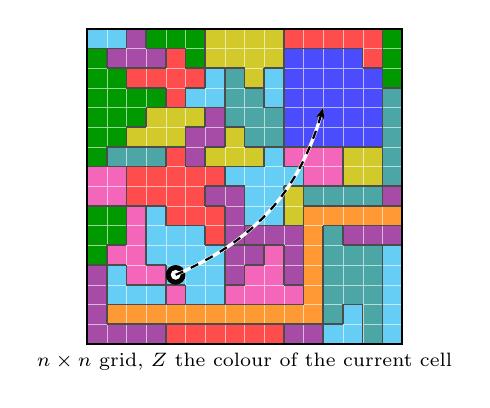
\begin{tikzpicture}[x=0.25cm, y=0.25cm]
  \fill[violet!70] (0,0) rectangle ++(1,1);
  \fill[violet!70] (0,1) rectangle ++(1,1);
  \fill[violet!70] (0,2) rectangle ++(1,1);
  \fill[violet!70] (0,3) rectangle ++(1,1);
  \fill[green!60!black] (0,4) rectangle ++(1,1);
  \fill[green!60!black] (0,5) rectangle ++(1,1);
  \fill[green!60!black] (0,6) rectangle ++(1,1);
  \fill[magenta!60] (0,7) rectangle ++(1,1);
  \fill[magenta!60] (0,8) rectangle ++(1,1);
  \fill[green!60!black] (0,9) rectangle ++(1,1);
  \fill[green!60!black] (0,10) rectangle ++(1,1);
  \fill[green!60!black] (0,11) rectangle ++(1,1);
  \fill[green!60!black] (0,12) rectangle ++(1,1);
  \fill[green!60!black] (0,13) rectangle ++(1,1);
  \fill[green!60!black] (0,14) rectangle ++(1,1);
  \fill[cyan!60] (0,15) rectangle ++(1,1);
  \fill[violet!70] (1,0) rectangle ++(1,1);
  \fill[orange!80] (1,1) rectangle ++(1,1);
  \fill[cyan!60] (1,2) rectangle ++(1,1);
  \fill[cyan!60] (1,3) rectangle ++(1,1);
  \fill[magenta!60] (1,4) rectangle ++(1,1);
  \fill[green!60!black] (1,5) rectangle ++(1,1);
  \fill[green!60!black] (1,6) rectangle ++(1,1);
  \fill[magenta!60] (1,7) rectangle ++(1,1);
  \fill[magenta!60] (1,8) rectangle ++(1,1);
  \fill[teal!70] (1,9) rectangle ++(1,1);
  \fill[green!60!black] (1,10) rectangle ++(1,1);
  \fill[green!60!black] (1,11) rectangle ++(1,1);
  \fill[green!60!black] (1,12) rectangle ++(1,1);
  \fill[green!60!black] (1,13) rectangle ++(1,1);
  \fill[violet!70] (1,14) rectangle ++(1,1);
  \fill[cyan!60] (1,15) rectangle ++(1,1);
  \fill[violet!70] (2,0) rectangle ++(1,1);
  \fill[orange!80] (2,1) rectangle ++(1,1);
  \fill[cyan!60] (2,2) rectangle ++(1,1);
  \fill[magenta!60] (2,3) rectangle ++(1,1);
  \fill[magenta!60] (2,4) rectangle ++(1,1);
  \fill[magenta!60] (2,5) rectangle ++(1,1);
  \fill[magenta!60] (2,6) rectangle ++(1,1);
  \fill[red!70] (2,7) rectangle ++(1,1);
  \fill[red!70] (2,8) rectangle ++(1,1);
  \fill[teal!70] (2,9) rectangle ++(1,1);
  \fill[yellow!80!black] (2,10) rectangle ++(1,1);
  \fill[green!60!black] (2,11) rectangle ++(1,1);
  \fill[green!60!black] (2,12) rectangle ++(1,1);
  \fill[red!70] (2,13) rectangle ++(1,1);
  \fill[violet!70] (2,14) rectangle ++(1,1);
  \fill[violet!70] (2,15) rectangle ++(1,1);
  \fill[violet!70] (3,0) rectangle ++(1,1);
  \fill[orange!80] (3,1) rectangle ++(1,1);
  \fill[cyan!60] (3,2) rectangle ++(1,1);
  \fill[magenta!60] (3,3) rectangle ++(1,1);
  \fill[cyan!60] (3,4) rectangle ++(1,1);
  \fill[cyan!60] (3,5) rectangle ++(1,1);
  \fill[cyan!60] (3,6) rectangle ++(1,1);
  \fill[red!70] (3,7) rectangle ++(1,1);
  \fill[red!70] (3,8) rectangle ++(1,1);
  \fill[teal!70] (3,9) rectangle ++(1,1);
  \fill[yellow!80!black] (3,10) rectangle ++(1,1);
  \fill[yellow!80!black] (3,11) rectangle ++(1,1);
  \fill[green!60!black] (3,12) rectangle ++(1,1);
  \fill[red!70] (3,13) rectangle ++(1,1);
  \fill[violet!70] (3,14) rectangle ++(1,1);
  \fill[green!60!black] (3,15) rectangle ++(1,1);
  \fill[red!70] (4,0) rectangle ++(1,1);
  \fill[orange!80] (4,1) rectangle ++(1,1);
  \fill[magenta!60] (4,2) rectangle ++(1,1);
  \fill[cyan!60] (4,3) rectangle ++(1,1);
  \fill[cyan!60] (4,4) rectangle ++(1,1);
  \fill[cyan!60] (4,5) rectangle ++(1,1);
  \fill[red!70] (4,6) rectangle ++(1,1);
  \fill[red!70] (4,7) rectangle ++(1,1);
  \fill[red!70] (4,8) rectangle ++(1,1);
  \fill[red!70] (4,9) rectangle ++(1,1);
  \fill[yellow!80!black] (4,10) rectangle ++(1,1);
  \fill[yellow!80!black] (4,11) rectangle ++(1,1);
  \fill[red!70] (4,12) rectangle ++(1,1);
  \fill[red!70] (4,13) rectangle ++(1,1);
  \fill[red!70] (4,14) rectangle ++(1,1);
  \fill[green!60!black] (4,15) rectangle ++(1,1);
  \fill[red!70] (5,0) rectangle ++(1,1);
  \fill[orange!80] (5,1) rectangle ++(1,1);
  \fill[cyan!60] (5,2) rectangle ++(1,1);
  \fill[cyan!60] (5,3) rectangle ++(1,1);
  \fill[cyan!60] (5,4) rectangle ++(1,1);
  \fill[cyan!60] (5,5) rectangle ++(1,1);
  \fill[red!70] (5,6) rectangle ++(1,1);
  \fill[red!70] (5,7) rectangle ++(1,1);
  \fill[red!70] (5,8) rectangle ++(1,1);
  \fill[violet!70] (5,9) rectangle ++(1,1);
  \fill[violet!70] (5,10) rectangle ++(1,1);
  \fill[yellow!80!black] (5,11) rectangle ++(1,1);
  \fill[cyan!60] (5,12) rectangle ++(1,1);
  \fill[red!70] (5,13) rectangle ++(1,1);
  \fill[green!60!black] (5,14) rectangle ++(1,1);
  \fill[green!60!black] (5,15) rectangle ++(1,1);
  \fill[red!70] (6,0) rectangle ++(1,1);
  \fill[orange!80] (6,1) rectangle ++(1,1);
  \fill[cyan!60] (6,2) rectangle ++(1,1);
  \fill[cyan!60] (6,3) rectangle ++(1,1);
  \fill[cyan!60] (6,4) rectangle ++(1,1);
  \fill[red!70] (6,5) rectangle ++(1,1);
  \fill[red!70] (6,6) rectangle ++(1,1);
  \fill[violet!70] (6,7) rectangle ++(1,1);
  \fill[red!70] (6,8) rectangle ++(1,1);
  \fill[yellow!80!black] (6,9) rectangle ++(1,1);
  \fill[violet!70] (6,10) rectangle ++(1,1);
  \fill[violet!70] (6,11) rectangle ++(1,1);
  \fill[cyan!60] (6,12) rectangle ++(1,1);
  \fill[cyan!60] (6,13) rectangle ++(1,1);
  \fill[yellow!80!black] (6,14) rectangle ++(1,1);
  \fill[yellow!80!black] (6,15) rectangle ++(1,1);
  \fill[red!70] (7,0) rectangle ++(1,1);
  \fill[orange!80] (7,1) rectangle ++(1,1);
  \fill[magenta!60] (7,2) rectangle ++(1,1);
  \fill[violet!70] (7,3) rectangle ++(1,1);
  \fill[violet!70] (7,4) rectangle ++(1,1);
  \fill[violet!70] (7,5) rectangle ++(1,1);
  \fill[violet!70] (7,6) rectangle ++(1,1);
  \fill[violet!70] (7,7) rectangle ++(1,1);
  \fill[cyan!60] (7,8) rectangle ++(1,1);
  \fill[yellow!80!black] (7,9) rectangle ++(1,1);
  \fill[yellow!80!black] (7,10) rectangle ++(1,1);
  \fill[teal!70] (7,11) rectangle ++(1,1);
  \fill[teal!70] (7,12) rectangle ++(1,1);
  \fill[teal!70] (7,13) rectangle ++(1,1);
  \fill[yellow!80!black] (7,14) rectangle ++(1,1);
  \fill[yellow!80!black] (7,15) rectangle ++(1,1);
  \fill[red!70] (8,0) rectangle ++(1,1);
  \fill[orange!80] (8,1) rectangle ++(1,1);
  \fill[magenta!60] (8,2) rectangle ++(1,1);
  \fill[magenta!60] (8,3) rectangle ++(1,1);
  \fill[violet!70] (8,4) rectangle ++(1,1);
  \fill[violet!70] (8,5) rectangle ++(1,1);
  \fill[cyan!60] (8,6) rectangle ++(1,1);
  \fill[cyan!60] (8,7) rectangle ++(1,1);
  \fill[cyan!60] (8,8) rectangle ++(1,1);
  \fill[yellow!80!black] (8,9) rectangle ++(1,1);
  \fill[teal!70] (8,10) rectangle ++(1,1);
  \fill[teal!70] (8,11) rectangle ++(1,1);
  \fill[teal!70] (8,12) rectangle ++(1,1);
  \fill[yellow!80!black] (8,13) rectangle ++(1,1);
  \fill[yellow!80!black] (8,14) rectangle ++(1,1);
  \fill[yellow!80!black] (8,15) rectangle ++(1,1);
  \fill[red!70] (9,0) rectangle ++(1,1);
  \fill[orange!80] (9,1) rectangle ++(1,1);
  \fill[magenta!60] (9,2) rectangle ++(1,1);
  \fill[magenta!60] (9,3) rectangle ++(1,1);
  \fill[magenta!60] (9,4) rectangle ++(1,1);
  \fill[violet!70] (9,5) rectangle ++(1,1);
  \fill[cyan!60] (9,6) rectangle ++(1,1);
  \fill[cyan!60] (9,7) rectangle ++(1,1);
  \fill[cyan!60] (9,8) rectangle ++(1,1);
  \fill[cyan!60] (9,9) rectangle ++(1,1);
  \fill[teal!70] (9,10) rectangle ++(1,1);
  \fill[teal!70] (9,11) rectangle ++(1,1);
  \fill[cyan!60] (9,12) rectangle ++(1,1);
  \fill[cyan!60] (9,13) rectangle ++(1,1);
  \fill[yellow!80!black] (9,14) rectangle ++(1,1);
  \fill[yellow!80!black] (9,15) rectangle ++(1,1);
  \fill[violet!70] (10,0) rectangle ++(1,1);
  \fill[orange!80] (10,1) rectangle ++(1,1);
  \fill[magenta!60] (10,2) rectangle ++(1,1);
  \fill[violet!70] (10,3) rectangle ++(1,1);
  \fill[violet!70] (10,4) rectangle ++(1,1);
  \fill[violet!70] (10,5) rectangle ++(1,1);
  \fill[yellow!80!black] (10,6) rectangle ++(1,1);
  \fill[yellow!80!black] (10,7) rectangle ++(1,1);
  \fill[cyan!60] (10,8) rectangle ++(1,1);
  \fill[magenta!60] (10,9) rectangle ++(1,1);
  \fill[blue!70] (10,10) rectangle ++(1,1);
  \fill[blue!70] (10,11) rectangle ++(1,1);
  \fill[blue!70] (10,12) rectangle ++(1,1);
  \fill[blue!70] (10,13) rectangle ++(1,1);
  \fill[blue!70] (10,14) rectangle ++(1,1);
  \fill[red!70] (10,15) rectangle ++(1,1);
  \fill[violet!70] (11,0) rectangle ++(1,1);
  \fill[orange!80] (11,1) rectangle ++(1,1);
  \fill[orange!80] (11,2) rectangle ++(1,1);
  \fill[orange!80] (11,3) rectangle ++(1,1);
  \fill[orange!80] (11,4) rectangle ++(1,1);
  \fill[orange!80] (11,5) rectangle ++(1,1);
  \fill[orange!80] (11,6) rectangle ++(1,1);
  \fill[teal!70] (11,7) rectangle ++(1,1);
  \fill[magenta!60] (11,8) rectangle ++(1,1);
  \fill[magenta!60] (11,9) rectangle ++(1,1);
  \fill[blue!70] (11,10) rectangle ++(1,1);
  \fill[blue!70] (11,11) rectangle ++(1,1);
  \fill[blue!70] (11,12) rectangle ++(1,1);
  \fill[blue!70] (11,13) rectangle ++(1,1);
  \fill[blue!70] (11,14) rectangle ++(1,1);
  \fill[red!70] (11,15) rectangle ++(1,1);
  \fill[cyan!60] (12,0) rectangle ++(1,1);
  \fill[teal!70] (12,1) rectangle ++(1,1);
  \fill[teal!70] (12,2) rectangle ++(1,1);
  \fill[teal!70] (12,3) rectangle ++(1,1);
  \fill[teal!70] (12,4) rectangle ++(1,1);
  \fill[teal!70] (12,5) rectangle ++(1,1);
  \fill[orange!80] (12,6) rectangle ++(1,1);
  \fill[teal!70] (12,7) rectangle ++(1,1);
  \fill[magenta!60] (12,8) rectangle ++(1,1);
  \fill[magenta!60] (12,9) rectangle ++(1,1);
  \fill[blue!70] (12,10) rectangle ++(1,1);
  \fill[blue!70] (12,11) rectangle ++(1,1);
  \fill[blue!70] (12,12) rectangle ++(1,1);
  \fill[blue!70] (12,13) rectangle ++(1,1);
  \fill[blue!70] (12,14) rectangle ++(1,1);
  \fill[red!70] (12,15) rectangle ++(1,1);
  \fill[cyan!60] (13,0) rectangle ++(1,1);
  \fill[cyan!60] (13,1) rectangle ++(1,1);
  \fill[teal!70] (13,2) rectangle ++(1,1);
  \fill[teal!70] (13,3) rectangle ++(1,1);
  \fill[teal!70] (13,4) rectangle ++(1,1);
  \fill[violet!70] (13,5) rectangle ++(1,1);
  \fill[orange!80] (13,6) rectangle ++(1,1);
  \fill[teal!70] (13,7) rectangle ++(1,1);
  \fill[yellow!80!black] (13,8) rectangle ++(1,1);
  \fill[yellow!80!black] (13,9) rectangle ++(1,1);
  \fill[blue!70] (13,10) rectangle ++(1,1);
  \fill[blue!70] (13,11) rectangle ++(1,1);
  \fill[blue!70] (13,12) rectangle ++(1,1);
  \fill[blue!70] (13,13) rectangle ++(1,1);
  \fill[blue!70] (13,14) rectangle ++(1,1);
  \fill[red!70] (13,15) rectangle ++(1,1);
  \fill[teal!70] (14,0) rectangle ++(1,1);
  \fill[teal!70] (14,1) rectangle ++(1,1);
  \fill[teal!70] (14,2) rectangle ++(1,1);
  \fill[teal!70] (14,3) rectangle ++(1,1);
  \fill[teal!70] (14,4) rectangle ++(1,1);
  \fill[violet!70] (14,5) rectangle ++(1,1);
  \fill[orange!80] (14,6) rectangle ++(1,1);
  \fill[teal!70] (14,7) rectangle ++(1,1);
  \fill[yellow!80!black] (14,8) rectangle ++(1,1);
  \fill[yellow!80!black] (14,9) rectangle ++(1,1);
  \fill[blue!70] (14,10) rectangle ++(1,1);
  \fill[blue!70] (14,11) rectangle ++(1,1);
  \fill[blue!70] (14,12) rectangle ++(1,1);
  \fill[blue!70] (14,13) rectangle ++(1,1);
  \fill[red!70] (14,14) rectangle ++(1,1);
  \fill[red!70] (14,15) rectangle ++(1,1);
  \fill[cyan!60] (15,0) rectangle ++(1,1);
  \fill[cyan!60] (15,1) rectangle ++(1,1);
  \fill[cyan!60] (15,2) rectangle ++(1,1);
  \fill[cyan!60] (15,3) rectangle ++(1,1);
  \fill[cyan!60] (15,4) rectangle ++(1,1);
  \fill[violet!70] (15,5) rectangle ++(1,1);
  \fill[orange!80] (15,6) rectangle ++(1,1);
  \fill[violet!70] (15,7) rectangle ++(1,1);
  \fill[teal!70] (15,8) rectangle ++(1,1);
  \fill[teal!70] (15,9) rectangle ++(1,1);
  \fill[teal!70] (15,10) rectangle ++(1,1);
  \fill[teal!70] (15,11) rectangle ++(1,1);
  \fill[teal!70] (15,12) rectangle ++(1,1);
  \fill[green!60!black] (15,13) rectangle ++(1,1);
  \fill[green!60!black] (15,14) rectangle ++(1,1);
  \fill[green!60!black] (15,15) rectangle ++(1,1);
  \draw[white, ultra thin, opacity=0.6, xstep=0.25cm, ystep=0.25cm] (0,0) grid (16,16);
  \draw[black!70, semithick] (1,1) -- ++(0,1);
  \draw[black!70, semithick] (1,2) -- ++(0,1);
  \draw[black!70, semithick] (1,3) -- ++(0,1);
  \draw[black!70, semithick] (0,4) -- ++(1,0);
  \draw[black!70, semithick] (1,4) -- ++(0,1);
  \draw[black!70, semithick] (0,7) -- ++(1,0);
  \draw[black!70, semithick] (0,9) -- ++(1,0);
  \draw[black!70, semithick] (1,9) -- ++(0,1);
  \draw[black!70, semithick] (1,14) -- ++(0,1);
  \draw[black!70, semithick] (0,15) -- ++(1,0);
  \draw[black!70, semithick] (1,1) -- ++(1,0);
  \draw[black!70, semithick] (1,2) -- ++(1,0);
  \draw[black!70, semithick] (2,3) -- ++(0,1);
  \draw[black!70, semithick] (1,4) -- ++(1,0);
  \draw[black!70, semithick] (1,5) -- ++(1,0);
  \draw[black!70, semithick] (2,5) -- ++(0,1);
  \draw[black!70, semithick] (2,6) -- ++(0,1);
  \draw[black!70, semithick] (1,7) -- ++(1,0);
  \draw[black!70, semithick] (2,7) -- ++(0,1);
  \draw[black!70, semithick] (2,8) -- ++(0,1);
  \draw[black!70, semithick] (1,9) -- ++(1,0);
  \draw[black!70, semithick] (1,10) -- ++(1,0);
  \draw[black!70, semithick] (2,10) -- ++(0,1);
  \draw[black!70, semithick] (2,13) -- ++(0,1);
  \draw[black!70, semithick] (1,14) -- ++(1,0);
  \draw[black!70, semithick] (1,15) -- ++(1,0);
  \draw[black!70, semithick] (2,15) -- ++(0,1);
  \draw[black!70, semithick] (2,1) -- ++(1,0);
  \draw[black!70, semithick] (2,2) -- ++(1,0);
  \draw[black!70, semithick] (2,3) -- ++(1,0);
  \draw[black!70, semithick] (3,4) -- ++(0,1);
  \draw[black!70, semithick] (3,5) -- ++(0,1);
  \draw[black!70, semithick] (3,6) -- ++(0,1);
  \draw[black!70, semithick] (2,7) -- ++(1,0);
  \draw[black!70, semithick] (2,9) -- ++(1,0);
  \draw[black!70, semithick] (2,10) -- ++(1,0);
  \draw[black!70, semithick] (2,11) -- ++(1,0);
  \draw[black!70, semithick] (3,11) -- ++(0,1);
  \draw[black!70, semithick] (2,13) -- ++(1,0);
  \draw[black!70, semithick] (2,14) -- ++(1,0);
  \draw[black!70, semithick] (3,15) -- ++(0,1);
  \draw[black!70, semithick] (4,0) -- ++(0,1);
  \draw[black!70, semithick] (3,1) -- ++(1,0);
  \draw[black!70, semithick] (3,2) -- ++(1,0);
  \draw[black!70, semithick] (4,2) -- ++(0,1);
  \draw[black!70, semithick] (3,3) -- ++(1,0);
  \draw[black!70, semithick] (4,3) -- ++(0,1);
  \draw[black!70, semithick] (3,4) -- ++(1,0);
  \draw[black!70, semithick] (4,6) -- ++(0,1);
  \draw[black!70, semithick] (3,7) -- ++(1,0);
  \draw[black!70, semithick] (3,9) -- ++(1,0);
  \draw[black!70, semithick] (4,9) -- ++(0,1);
  \draw[black!70, semithick] (3,10) -- ++(1,0);
  \draw[black!70, semithick] (3,12) -- ++(1,0);
  \draw[black!70, semithick] (4,12) -- ++(0,1);
  \draw[black!70, semithick] (3,13) -- ++(1,0);
  \draw[black!70, semithick] (3,14) -- ++(1,0);
  \draw[black!70, semithick] (4,14) -- ++(0,1);
  \draw[black!70, semithick] (3,15) -- ++(1,0);
  \draw[black!70, semithick] (4,1) -- ++(1,0);
  \draw[black!70, semithick] (4,2) -- ++(1,0);
  \draw[black!70, semithick] (5,2) -- ++(0,1);
  \draw[black!70, semithick] (4,3) -- ++(1,0);
  \draw[black!70, semithick] (4,6) -- ++(1,0);
  \draw[black!70, semithick] (5,9) -- ++(0,1);
  \draw[black!70, semithick] (4,10) -- ++(1,0);
  \draw[black!70, semithick] (5,10) -- ++(0,1);
  \draw[black!70, semithick] (4,12) -- ++(1,0);
  \draw[black!70, semithick] (5,12) -- ++(0,1);
  \draw[black!70, semithick] (5,14) -- ++(0,1);
  \draw[black!70, semithick] (4,15) -- ++(1,0);
  \draw[black!70, semithick] (5,1) -- ++(1,0);
  \draw[black!70, semithick] (5,2) -- ++(1,0);
  \draw[black!70, semithick] (6,5) -- ++(0,1);
  \draw[black!70, semithick] (5,6) -- ++(1,0);
  \draw[black!70, semithick] (6,7) -- ++(0,1);
  \draw[black!70, semithick] (5,9) -- ++(1,0);
  \draw[black!70, semithick] (6,9) -- ++(0,1);
  \draw[black!70, semithick] (5,11) -- ++(1,0);
  \draw[black!70, semithick] (6,11) -- ++(0,1);
  \draw[black!70, semithick] (5,12) -- ++(1,0);
  \draw[black!70, semithick] (5,13) -- ++(1,0);
  \draw[black!70, semithick] (6,13) -- ++(0,1);
  \draw[black!70, semithick] (5,14) -- ++(1,0);
  \draw[black!70, semithick] (6,14) -- ++(0,1);
  \draw[black!70, semithick] (6,15) -- ++(0,1);
  \draw[black!70, semithick] (6,1) -- ++(1,0);
  \draw[black!70, semithick] (6,2) -- ++(1,0);
  \draw[black!70, semithick] (7,2) -- ++(0,1);
  \draw[black!70, semithick] (7,3) -- ++(0,1);
  \draw[black!70, semithick] (7,4) -- ++(0,1);
  \draw[black!70, semithick] (6,5) -- ++(1,0);
  \draw[black!70, semithick] (7,5) -- ++(0,1);
  \draw[black!70, semithick] (7,6) -- ++(0,1);
  \draw[black!70, semithick] (6,7) -- ++(1,0);
  \draw[black!70, semithick] (6,8) -- ++(1,0);
  \draw[black!70, semithick] (7,8) -- ++(0,1);
  \draw[black!70, semithick] (6,9) -- ++(1,0);
  \draw[black!70, semithick] (6,10) -- ++(1,0);
  \draw[black!70, semithick] (7,10) -- ++(0,1);
  \draw[black!70, semithick] (7,11) -- ++(0,1);
  \draw[black!70, semithick] (6,12) -- ++(1,0);
  \draw[black!70, semithick] (7,12) -- ++(0,1);
  \draw[black!70, semithick] (7,13) -- ++(0,1);
  \draw[black!70, semithick] (6,14) -- ++(1,0);
  \draw[black!70, semithick] (7,1) -- ++(1,0);
  \draw[black!70, semithick] (7,2) -- ++(1,0);
  \draw[black!70, semithick] (7,3) -- ++(1,0);
  \draw[black!70, semithick] (8,3) -- ++(0,1);
  \draw[black!70, semithick] (7,5) -- ++(1,0);
  \draw[black!70, semithick] (8,5) -- ++(0,1);
  \draw[black!70, semithick] (8,6) -- ++(0,1);
  \draw[black!70, semithick] (8,7) -- ++(0,1);
  \draw[black!70, semithick] (7,8) -- ++(1,0);
  \draw[black!70, semithick] (7,9) -- ++(1,0);
  \draw[black!70, semithick] (8,10) -- ++(0,1);
  \draw[black!70, semithick] (7,11) -- ++(1,0);
  \draw[black!70, semithick] (8,13) -- ++(0,1);
  \draw[black!70, semithick] (7,14) -- ++(1,0);
  \draw[black!70, semithick] (8,1) -- ++(1,0);
  \draw[black!70, semithick] (8,2) -- ++(1,0);
  \draw[black!70, semithick] (8,4) -- ++(1,0);
  \draw[black!70, semithick] (9,4) -- ++(0,1);
  \draw[black!70, semithick] (8,5) -- ++(1,0);
  \draw[black!70, semithick] (8,6) -- ++(1,0);
  \draw[black!70, semithick] (8,9) -- ++(1,0);
  \draw[black!70, semithick] (9,9) -- ++(0,1);
  \draw[black!70, semithick] (8,10) -- ++(1,0);
  \draw[black!70, semithick] (9,12) -- ++(0,1);
  \draw[black!70, semithick] (8,13) -- ++(1,0);
  \draw[black!70, semithick] (9,13) -- ++(0,1);
  \draw[black!70, semithick] (10,0) -- ++(0,1);
  \draw[black!70, semithick] (9,1) -- ++(1,0);
  \draw[black!70, semithick] (9,2) -- ++(1,0);
  \draw[black!70, semithick] (10,3) -- ++(0,1);
  \draw[black!70, semithick] (10,4) -- ++(0,1);
  \draw[black!70, semithick] (9,5) -- ++(1,0);
  \draw[black!70, semithick] (9,6) -- ++(1,0);
  \draw[black!70, semithick] (10,6) -- ++(0,1);
  \draw[black!70, semithick] (10,7) -- ++(0,1);
  \draw[black!70, semithick] (10,9) -- ++(0,1);
  \draw[black!70, semithick] (9,10) -- ++(1,0);
  \draw[black!70, semithick] (10,10) -- ++(0,1);
  \draw[black!70, semithick] (10,11) -- ++(0,1);
  \draw[black!70, semithick] (9,12) -- ++(1,0);
  \draw[black!70, semithick] (10,12) -- ++(0,1);
  \draw[black!70, semithick] (10,13) -- ++(0,1);
  \draw[black!70, semithick] (9,14) -- ++(1,0);
  \draw[black!70, semithick] (10,14) -- ++(0,1);
  \draw[black!70, semithick] (10,15) -- ++(0,1);
  \draw[black!70, semithick] (10,1) -- ++(1,0);
  \draw[black!70, semithick] (10,2) -- ++(1,0);
  \draw[black!70, semithick] (11,2) -- ++(0,1);
  \draw[black!70, semithick] (10,3) -- ++(1,0);
  \draw[black!70, semithick] (11,3) -- ++(0,1);
  \draw[black!70, semithick] (11,4) -- ++(0,1);
  \draw[black!70, semithick] (11,5) -- ++(0,1);
  \draw[black!70, semithick] (10,6) -- ++(1,0);
  \draw[black!70, semithick] (11,6) -- ++(0,1);
  \draw[black!70, semithick] (11,7) -- ++(0,1);
  \draw[black!70, semithick] (10,8) -- ++(1,0);
  \draw[black!70, semithick] (11,8) -- ++(0,1);
  \draw[black!70, semithick] (10,9) -- ++(1,0);
  \draw[black!70, semithick] (10,10) -- ++(1,0);
  \draw[black!70, semithick] (10,15) -- ++(1,0);
  \draw[black!70, semithick] (12,0) -- ++(0,1);
  \draw[black!70, semithick] (11,1) -- ++(1,0);
  \draw[black!70, semithick] (12,1) -- ++(0,1);
  \draw[black!70, semithick] (12,2) -- ++(0,1);
  \draw[black!70, semithick] (12,3) -- ++(0,1);
  \draw[black!70, semithick] (12,4) -- ++(0,1);
  \draw[black!70, semithick] (12,5) -- ++(0,1);
  \draw[black!70, semithick] (11,7) -- ++(1,0);
  \draw[black!70, semithick] (11,8) -- ++(1,0);
  \draw[black!70, semithick] (11,10) -- ++(1,0);
  \draw[black!70, semithick] (11,15) -- ++(1,0);
  \draw[black!70, semithick] (12,1) -- ++(1,0);
  \draw[black!70, semithick] (13,1) -- ++(0,1);
  \draw[black!70, semithick] (13,5) -- ++(0,1);
  \draw[black!70, semithick] (12,6) -- ++(1,0);
  \draw[black!70, semithick] (12,7) -- ++(1,0);
  \draw[black!70, semithick] (12,8) -- ++(1,0);
  \draw[black!70, semithick] (13,8) -- ++(0,1);
  \draw[black!70, semithick] (13,9) -- ++(0,1);
  \draw[black!70, semithick] (12,10) -- ++(1,0);
  \draw[black!70, semithick] (12,15) -- ++(1,0);
  \draw[black!70, semithick] (14,0) -- ++(0,1);
  \draw[black!70, semithick] (14,1) -- ++(0,1);
  \draw[black!70, semithick] (13,2) -- ++(1,0);
  \draw[black!70, semithick] (13,5) -- ++(1,0);
  \draw[black!70, semithick] (13,6) -- ++(1,0);
  \draw[black!70, semithick] (13,7) -- ++(1,0);
  \draw[black!70, semithick] (13,8) -- ++(1,0);
  \draw[black!70, semithick] (13,10) -- ++(1,0);
  \draw[black!70, semithick] (14,14) -- ++(0,1);
  \draw[black!70, semithick] (13,15) -- ++(1,0);
  \draw[black!70, semithick] (15,0) -- ++(0,1);
  \draw[black!70, semithick] (15,1) -- ++(0,1);
  \draw[black!70, semithick] (15,2) -- ++(0,1);
  \draw[black!70, semithick] (15,3) -- ++(0,1);
  \draw[black!70, semithick] (15,4) -- ++(0,1);
  \draw[black!70, semithick] (14,5) -- ++(1,0);
  \draw[black!70, semithick] (14,6) -- ++(1,0);
  \draw[black!70, semithick] (14,7) -- ++(1,0);
  \draw[black!70, semithick] (15,7) -- ++(0,1);
  \draw[black!70, semithick] (14,8) -- ++(1,0);
  \draw[black!70, semithick] (15,8) -- ++(0,1);
  \draw[black!70, semithick] (15,9) -- ++(0,1);
  \draw[black!70, semithick] (14,10) -- ++(1,0);
  \draw[black!70, semithick] (15,10) -- ++(0,1);
  \draw[black!70, semithick] (15,11) -- ++(0,1);
  \draw[black!70, semithick] (15,12) -- ++(0,1);
  \draw[black!70, semithick] (15,13) -- ++(0,1);
  \draw[black!70, semithick] (14,14) -- ++(1,0);
  \draw[black!70, semithick] (15,14) -- ++(0,1);
  \draw[black!70, semithick] (15,15) -- ++(0,1);
  \draw[black!70, semithick] (15,5) -- ++(1,0);
  \draw[black!70, semithick] (15,6) -- ++(1,0);
  \draw[black!70, semithick] (15,7) -- ++(1,0);
  \draw[black!70, semithick] (15,8) -- ++(1,0);
  \draw[black!70, semithick] (15,13) -- ++(1,0);
  \draw[thick] (0,0) rectangle (16,16);
  \fill[black] (4.5,3.5) circle (0.5);
  \fill[white] (4.5,3.5) circle (0.25);
  \draw[-{Stealth[length=1.5mm]}, very thick, white] (4.5,3.5) to[bend right=25] (12,12);
  \draw[-{Stealth[length=1.5mm]}, thick, black, dashed] (4.5,3.5) to[bend right=25] (12,12);
  \node[below, font=\scriptsize] at (8,0) {$n \times n$ grid, $Z$ the colour of the current cell};
\end{tikzpicture}
\end{minipage}\hfill
\begin{minipage}[c]{0.5\textwidth}\centering\stubplot{round $k$}{$H(\psi_\# d^{\pi_k})$}\end{minipage}
\caption{Colour grid. Left, a grid packed with polyomino tiles, where the thin orange tile has the most cells and the compact blue tile is the most stable. Right, outcome entropy over the rounds, placeholder.}
\label{fig:colourgrid}
\end{figure}

\paragraph{Cart-pole, continuous outcomes.}
\intent{Barto dynamics, $Z$ the pole angle on the circle, $\lambda$ Lebesgue, kicks on the angular velocity, MM with a kernel estimate $\hat q$ and MPPI, 8 seeds.
Claim: the criterion balances with no reward and the spread grows with the kick, the dark room at $\nu = \lambda$ from hanging with the crossover $\beta_0 \approx 0.52$ of Proposition~\ref{prop:alignment}, and swing-up fails below $\beta \approx 16$ because the refit $\hat q$ builds a barrier at the start state, which is the estimation gap of Proposition~\ref{prop:plugin}.}
\todo{Figure: angle histograms against $\nu$, success against $\beta$, the barrier in $-\ln \hat q$; test the $\epsilon$-mixing fix.}

\begin{figure}[h]
\centering
\begin{minipage}[c]{0.45\textwidth}\centering% Cart-pole, schematic. Z is the pole angle on the circle, kicks act on the angular velocity.
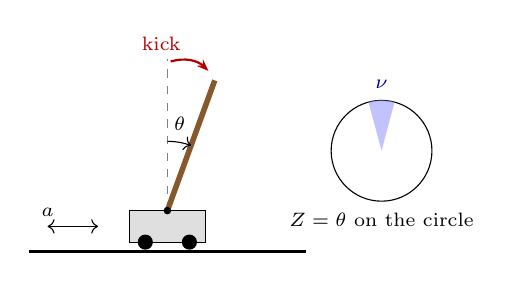
\begin{tikzpicture}[scale=0.8]
  \draw[thick] (-2.2,0) -- (2.2,0);
  \fill[gray!25, draw=black] (-0.6,0.15) rectangle (0.6,0.65);
  \fill[black] (-0.35,0.15) circle (0.12) (0.35,0.15) circle (0.12);
  \coordinate (pivot) at (0,0.65);
  \coordinate (tip) at ($(pivot)+(70:2.2)$);
  \draw[dashed, gray] (pivot) -- ++(0,2.4);
  \draw[line width=2pt, brown!70!black] (pivot) -- (tip);
  \fill[black] (pivot) circle (0.06);
  \draw[->] ($(pivot)+(0,1.1)$) arc (90:70:1.1);
  \node[font=\scriptsize] at ($(pivot)+(82:1.4)$) {$\theta$};
  \draw[-{Stealth[length=1.5mm]}, red!70!black, thick] ($(tip)+(-0.7,0.3)$) to[bend left=30] node[above left, font=\scriptsize] {kick} ($(tip)+(-0.1,0.15)$);
  \draw[<->] (-1.1,0.4) -- (-1.9,0.4) node[above, font=\scriptsize] {$a$};
  % outcome circle with nu
  \begin{scope}[shift={(3.4,1.6)}]
    \draw (0,0) circle (0.8);
    \fill[blue!40, opacity=0.6] (0,0) -- (75:0.8) arc (75:105:0.8) -- cycle;
    \node[font=\scriptsize] at (0,-1.1) {$Z = \theta$ on the circle};
    \node[font=\scriptsize, blue!60!black] at (0,1.05) {$\nu$};
  \end{scope}
\end{tikzpicture}
\end{minipage}\hfill
\begin{minipage}[c]{0.5\textwidth}\centering\stubplot{$\beta$}{swing-up success}\end{minipage}
\caption{Cart-pole. Left, the pole angle $\theta$ is the outcome on the circle, kicked on its angular velocity, with $\nu$ concentrated upright. Right, success against $\beta$, placeholder.}
\label{fig:cartpole}
\end{figure}

\paragraph{DeepSea, the law floor.}
\intent{DeepSea \citep{Osband-behaviour20} with $P$ known and the reward channel $\kappa$ unknown, exact DP on the DAG per episode, 16 seeds, $L \in \{10, 20, 30\}$.
Claim: the bare criterion collapses on a finite belief, and the law floor with the seeking sign rescues it. Beta posterior never collapses, finite belief collapses at a single episode, averse law term 0/16, seeking $\lambda_\kappa = 5$ 16/16, capped $\lambda_\kappa \le 4$ no rescue, threshold between 4 and 5 unresolved. Action empowerment at either level only acts as a temperature.}
\todo{Figure: depth reached per episode for bare, averse and seeking; resolve the $\lambda_\kappa$ threshold.}

\begin{figure}[h]
\centering
\begin{minipage}[c]{0.45\textwidth}\centering% DeepSea of depth L, schematic. Row t is time, the agent moves one row down per step, left or right.
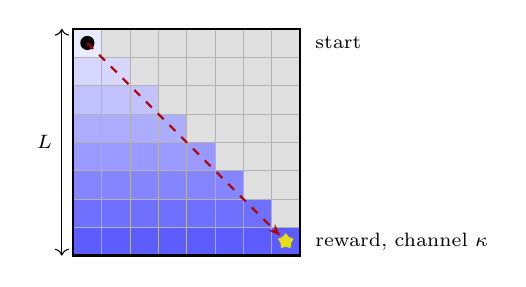
\begin{tikzpicture}[x=0.36cm, y=0.36cm]
  \def\L{8}
  \foreach \r in {0,...,7} {
    \foreach \c in {0,...,7} {
      \pgfmathparse{\c > \r ? 1 : 0}
      \ifnum\pgfmathresult=1
        \fill[gray!25] (\c,-\r) rectangle ++(1,-1);
      \else
        \fill[blue!\the\numexpr 8+8*\r\relax] (\c,-\r) rectangle ++(1,-1);
      \fi
    }
  }
  \draw[gray!60, very thin, xstep=0.36cm, ystep=0.36cm] (0,0) grid (8,-8);
  \draw[thick] (0,0) rectangle (8,-8);
  \fill[black] (0.5,-0.5) circle (0.25);
  \node[star, star points=5, fill=yellow!90!black, inner sep=1.4pt] at (7.5,-7.5) {};
  \draw[-{Stealth[length=1.5mm]}, thick, dashed, red!70!black] (0.5,-0.5) -- (7.3,-7.3);
  \node[font=\scriptsize, anchor=west] at (8.2,-0.5) {start};
  \node[font=\scriptsize, anchor=west] at (8.2,-7.5) {reward, channel $\kappa$};
  \draw[<->] (-0.4,0) -- (-0.4,-8) node[midway, left, font=\scriptsize] {$L$};
\end{tikzpicture}
\end{minipage}\hfill
\begin{minipage}[c]{0.5\textwidth}\centering\stubplot{episode}{depth reached}\end{minipage}
\caption{DeepSea of depth $L$. Left, each step moves one row down and left or right, the reward sits at the far corner behind an unknown channel $\kappa$. Right, depth reached per episode for the bare, averse and seeking law terms, placeholder.}
\label{fig:deepsea}
\end{figure}

\intent{Open examples from the planning notes, a two-goal maze, constrained permutation under random durations, and the SMiRL comparison, named in one line if space allows.}

% !TEX root = ../main.tex
%%%%%%%%%%%%%%%%%%%%%%%%%%%%%%%%%%%%%%%%%%%%%%%%%%%%%%%%%%%%%%%%
\section[Discussion and related work]{Discussion and related work \budget{1.5 pp}}
\label{sec:related}
\label{sec:discussion}

\add{Supplementary~\ref{sup:related} extends each paragraph.}

\paragraph{\add{Predictability objectives.}}
\add{Predictability has been an objective as the entropy rate of the state process \citep{JarneOrnia-predictable25,vanZutphen-predictable24}, as the entropy of the output in minimum-entropy control \citep{Wang-minimum02}, as the surprise of the agent's own states under a density refit within the episode \citep{Berseth-smirl21}, and as motion that matches what a human observer expects \citep{Dragan-legibility13}.}
\add{These score predictability step by step, within one trajectory, or in the eyes of an observer.}
\add{The pooled outcome entropy itself is stated as an ergodic sensory entropy by \citet{Friston-free12c} and minimised open loop by \citet{Adurthi-minimum14}, while \citet{Wang-minimum02} minimises the entropy of the output one step ahead.}

\paragraph{\add{Free energy principle and active inference.}}
\add{The free energy principle states our aim for the sensory states, a system that minimises the long-run entropy of its sensations through a deterministic internal map \citep{Friston-free12c}, and its descent step freezes the sensory density at the model, which is the inner step of \eqref{eq:game} without the refit \citep{Friston-free12b}.}
\add{Determinism is assumed there, while Theorem~\ref{thm:criterion} derives it from the concavity of the criterion.}
\add{Active inference plans with the expected free energy instead, which penalises the ambiguity of outcomes given hidden states but rewards the information outcomes carry about those states, the opposite sign to our criterion on both the outcome entropy and the information terms \citep{Friston-active15}.}
\add{Our floors take the place of that reward, they buy the information that identifiability needs and go slack after it, where the expected free energy keeps seeking it.}

\paragraph{\add{Cybernetics and control.}}
\add{Ashby framed regulation as keeping the essential variables within limits \citep{Ashby-design60} and quantified it in the law of requisite variety, whose Shannon form $H(E) \ge H(D) + H_D(R) - H(R)$ bounds how far the regulator's own variety can lower that of the outcome and is tightest when the regulator's move is a function of the disturbance \citep[ch.~11]{Ashby-introduction56}.}
\add{Conant and Ashby replace the limits by the entropy of the outcome and show that its simplest minimiser is a model of the system \citep{Conant-good70}, and our floors are in the spirit of the requisite variety bound.}
\add{\citet{Wentworth-fixing21} shows that the model claim is lost once the regulator sees only a noisy view of the system, recovers it for expected utility as a deterministic function of the posterior, and with his gooder regulator, which must serve tasks revealed later at minimal memory, forces a model isomorphic to that posterior.}
\add{He leaves open whether this carries over to the entropy criterion, where Theorem~\ref{thm:criterion} gives a deterministic regulator on the belief and the floors supply the pressure to identify that his task uncertainty supplies.}
\add{\citet{Richens-general25} reach a model through competence instead, since an agent that achieves enough multi-step goals has a transition model that can be read off its policy, while myopic agents need none.}
\add{In control theory the internal model principle makes the model necessary, since a structurally stable controller that rejects a persistent exogenous signal must contain a copy of the system that generates it \citep{Francis-internal76}, and the model it forces is one of the disturbance rather than of the plant.}
\add{Internal model control and model predictive control place a model inside the controller by design \citep{Garcia-internal82,Mayne-constrained00}.}

\paragraph{Control as inference.}
\label{sec:cai}
\add{Control as inference writes optimality as a likelihood $e^{r}$ on trajectories and recovers RL as inference under it \citep{Levine-reinforcement18}.}
\add{Here the likelihood is the inverse volume ratio $\dd\lambda / \dd\nu = e^{r}$, so with $q = q_k$ the cost in \eqref{eq:game} is $-\ln \tilde q_k$ up to a constant, with $\tilde q_k \propto q_k\, e^{r}$ the outcome law conditioned on optimality, and the game is inference on outcomes, where $\nu$ may have infinite volume and a hard goal set makes optimality the event $Z \in G$.}
\add{Its bonus on the policy entropy comes from the action floor, clearest for $Z = (S,A)$ with counting $\lambda$, where noise and ambiguity vanish, the regulation term is $H(S)$ and the empowerment term is $H(A \mid S)$ under $\occ$, the normalised discounted sum of per-step policy entropies.}
\add{With $\ln \tfrac{\dd\nu}{\dd\lambda} = -\beta r$, $\lambda_A = 1 + \alpha\beta$ and $c_A \ge \ln|\Acal|$, so that the hinge in \eqref{eq:lagrangian} never goes slack, $\Lcal(\pi) = H(S) - \beta\big(\E_{\occ}[r] + \alpha H(A \mid S)\big)$ is the maximum entropy objective at temperature $\alpha$, scaled by $\beta$, plus the state entropy, and a non-uniform action prior folds into $r$ \citep[Sec.~2.3]{Levine-reinforcement18}.}
\add{Control as inference is thus the Lagrangian minus the regulation term rather than a special case, and no $\nu$ or floor absorbs the residual, since $\nu$ is linear in $\occ$ and the regulation term has no multiplier.}
\add{The floor sets the regime, as for $\lambda_A \le 1$ this $\Lcal$ is concave and Theorem~\ref{thm:criterion} keeps a deterministic minimiser, while for $\lambda_A > 1$ the action term is convex and the minimiser can be interior.}
\add{The loop of \eqref{eq:game} is the concave-convex procedure \citep{Yuille-concave03}, since by $H(p) + \KL(p \,\|\, q) = \E_p[-\ln q]$ each round minimises $\Lcal(\pi) + \KL(p_\pi \,\|\, q_k)$, which linearises the concave entropy at $q_k$ and keeps the convex floors exact, a proximal step with prior $q_k$ whose unit weight alone makes the round linear in the outcome law, so no step size is tuned.}
\add{For $Z = (S,A)$ this KL is on the joint occupancy as in relative entropy policy search \citep{Peters-relative10}, a mirror descent step on the linear reward with learning rate $\beta$ \citep[Sec.~5.1.1]{Neu-unified17}, and the chain rule splits it into a state cost $-\ln d_k(s)$ and the exact trust region $\E_{\occ}\KL(\pi \,\|\, \pi_k)$ under the new occupancy \citep[Sec.~5.1.2]{Neu-unified17}, which the expectation step of \citet{Abdolmaleki-maximum18} evaluates on replay states.}
\add{Each round is thus the soft MDP with reward $\beta r + \ln d_k(s,a)$ at temperature $\lambda_A$ and descends $\Lcal$, and as the KL has zero value and gradient at a fixed point, that point is a stationary point of the nonconvex $\Lcal$ and no more, at $\lambda_A = 1 + \alpha\beta$ the soft optimal policy at temperature $\alpha$ for $r + \beta^{-1} \ln d(s)$ under its own occupancy, so the state entropy shifts the soft optimum of control as inference.}
\add{At $\lambda_A = 0$ the reward $\ln d_k$ is $-\infty$ off the support of $d_k$, so every deterministic policy is a fixed point of an exact refit, which the mixing of Proposition~\ref{prop:plugin} removes.}
\add{For $Z = (S,A,S')$ the identity gains the transition noise $\E_{\occ}[H(P(\cdot \mid S,A))]$ with a positive sign, so the criterion charges for noise, whereas exact inference backs up $\log \E[e^{V}]$ and is optimistic about it \citep[Sec.~2.3]{Levine-reinforcement18}, and the variational form with fixed dynamics restores the expected backup and is neutral \citep[Sec.~3.1]{Levine-reinforcement18}.}

\intent{Discussion: which outcome to regulate as the abstraction question; limits; outlook.}


%%%%%%%%%%%%%%%%%%%%%%%%%%%%%%%%%%%%%%%%%%%%%%%%%%%%%%%%%%%%%%%%
% Appendices count toward the 8--12 page limit.
%%%%%%%%%%%%%%%%%%%%%%%%%%%%%%%%%%%%%%%%%%%%%%%%%%%%%%%%%%%%%%%%
\appendix
% !TEX root = ../main.tex
%%%%%%%%%%%%%%%%%%%%%%%%%%%%%%%%%%%%%%%%%%%%%%%%%%%%%%%%%%%%%%%%
\section{Proofs and environments}
\label{app:proofs}
\label{app:envs}
\label{app:experiments}
\intent{Environment details; proofs are in Supplementary~\ref{sup:proofs}.}


\bibliography{main}
\bibliographystyle{rlj}

\beginSupplementaryMaterials
% !TEX root =../main.tex
%%%%%%%%%%%%%%%%%%%%%%%%%%%%%%%%%%%%%%%%%%%%%%%%%%%%%%%%%%%%%%%%
\section{Proofs}
\label{sup:proofs}

Throughout, $\lambda$ is the base measure on $\Zcal$, all laws are absolutely continuous with respect to the references they are measured against, and conditional entropies are averaged over the conditioning variable.

\subsection{Proof of Theorem~\ref{thm:criterion}}
\label{sup:proof-criterion}
\emph{Identity.}
Given $\hat Z = k$ the event $Z$ has law $k$ by definition of the observable class, so $H_\rho(\hat Z) + H_\lambda(Z \mid \hat Z) = H_\lambda(Z) + H_\rho(\hat Z \mid Z)$, both sides being the entropy of the pair against $\rho \otimes \lambda$, whose density factorises in either order.
Part 1 of Proposition~\ref{prop:alignment} gives $H_\nu(Z) = H_\lambda(Z) + \E[\ell(Z)]$ with $\ell := \ln \tfrac{\dd\nu}{\dd\lambda}$, and substituting gives \eqref{eq:classes}.
The joint law of $(\hat Z, Z)$ is the law of $\hat Z$ with $Z \mid \hat Z = k \sim k$, so every term is a functional of the law of $\hat Z$.

\emph{Belief.}
The belief is the state of the belief MDP, which the history policy drives as a history policy \citep{Astrom-optimal65,Kaelbling-planning98}, so there is a Markov policy on the belief with the same marginal laws of $(b_t, A_t)$ for every $t$ \citep{Puterman-markov94}.
Since $\Pr(S_t = s, A_t = a) = \E[b_t(s)\, \mathbf 1\{A_t = a\}]$ is a functional of that marginal, the state-action occupancy and with it $\pz$ and $H_\nu(Z)$ are unchanged.
When the belief takes finitely many values the belief MDP is finite, its occupancy set is a polytope whose vertices are the deterministic stationary policies \citep{Derman-finite70ch7}, $\pz$ is linear in the occupancy and $H_\nu$ is concave, so a minimum is attained at a vertex.
\hfill$\square$

\subsection{Proof of Proposition~\ref{prop:alignment}}
\label{sup:proof-alignment}
\emph{Part 1.}
By the chain rule for Radon--Nikodym derivatives, $\tfrac{\dd p}{\dd\nu} = \tfrac{\dd p}{\dd\lambda} \tfrac{\dd\lambda}{\dd\nu}$, so $-\ln \tfrac{\dd p}{\dd\nu} = -\ln \tfrac{\dd p}{\dd\lambda} + \ln \tfrac{\dd\nu}{\dd\lambda}$.
Integrating against $p$ gives $H_\nu(p) = H_\lambda(p) + \E_p\big[\ln \tfrac{\dd\nu}{\dd\lambda}\big]$.

\emph{Part 2.}
Part 1 applied to $\nu_\beta$, with $\ln \tfrac{\dd\nu_\beta}{\dd\lambda} = \beta \ln \tfrac{\dd\nu}{\dd\lambda}$, gives $H_{\nu_\beta}(p) = H_\lambda(p) + \beta\, \E_p\big[\ln \tfrac{\dd\nu}{\dd\lambda}\big]$.

\emph{Part 3.}
For each $\beta$ the criterion $H_{\nu_\beta}$ is concave in the occupancy, because the event law is linear in it and $H_\lambda$ is concave while the second term is linear, so a minimiser exists among the finitely many vertices, the deterministic stationary policies.
Let $V$ be that finite set, $\pi_\nu \in V$ minimise $\E_\pi\big[\ln \tfrac{\dd\nu}{\dd\lambda}(Z)\big]$ with value $g^\star$, and $\delta > 0$ the smallest gap $\E_\pi\big[\ln \tfrac{\dd\nu}{\dd\lambda}(Z)\big] - g^\star$ over vertices $\pi$ with a strictly larger value.
On finite $\Zcal$ with counting $\lambda$, $0 \le H_\lambda \le \ln |\Zcal|$, so for $\beta > \beta_0 := \ln|\Zcal| / \delta$ the second term grows by more than $\beta\delta > \ln|\Zcal|$ on every vertex with a larger value, which puts its $H_{\nu_\beta}$ strictly above that of $\pi_\nu$.
Among the vertices that attain $g^\star$ the second term is the same constant, so they are ordered by $H_\lambda$ alone.
\hfill$\square$

\subsection{Proof of Corollary~\ref{prop:split}}
\label{sup:proof-split}
The direct proof follows, and the derivation from Proposition~\ref{prop:split-pomdp} is given in the main text.
Write $\ell := \ln \tfrac{\dd\nu}{\dd\lambda}$, so that Proposition~\ref{prop:alignment} reads $H_\nu(q) = H_\lambda(q) + \E_q[\ell]$ for every law $q$, in particular for the law of $Z$ given each class.
The left-hand side is fixed and each line names the step that produces it.
\begin{align*}
 H_\nu(Z) &= H_\lambda(Z) + \E[\ell(Z)] && \text{Proposition~\ref{prop:alignment}} \\
      &= H_\rho(\tilde Z) + H_\lambda(Z \mid \tilde Z) - H_\rho(\tilde Z \mid Z) + \E[\ell(Z)] && \text{chain rule on } (\tilde Z, Z) \text{, both orders} \\
      &= H_\rho(\tilde Z) + H_\nu(Z \mid \tilde Z) - H_\rho(\tilde Z \mid Z) && \text{Proposition~\ref{prop:alignment} given each class} \\
      &= I(S;\tilde Z) + I(A;\tilde Z \mid S) + H_\nu(Z \mid \tilde Z) - H_\rho(\tilde Z \mid Z) && \text{chain rule on } H_\rho(\tilde Z).
\end{align*}
The second line uses $H_\rho(\tilde Z) + H_\lambda(Z \mid \tilde Z) = H_\lambda(Z) + H_\rho(\tilde Z \mid Z)$, both sides being the entropy of the pair against $\rho \otimes \lambda$, whose density factorises in either order.
The third line uses $\E[\ell(Z)] = \E\big[\E[\ell(Z) \mid \tilde Z]\big]$.
The last line is the chain rule $H_\rho(\tilde Z) = I(S;\tilde Z) + I(A;\tilde Z \mid S) + H_\rho(\tilde Z \mid S,A)$ for counting $\rho$, whose residual is zero because $\tilde Z$ is a function of $(S,A)$.
\hfill$\square$

\subsection{Proof of Corollary~\ref{cor:freebits}}
\label{sup:proof-freebits}
Given $S = s$ the class $\kappa(s,A)$ is a function of $A$, and a function of $A$ is independent of $A$ exactly when it is constant on the support of $\pi(\cdot \mid s)$.
The identity is the definition of conditional mutual information, and by Corollary~\ref{prop:split} only $I(A;\tilde Z \mid S)$ enters the criterion.
\hfill$\square$

\subsection{Proof of Proposition~\ref{prop:split-pomdp}}
\label{sup:proof-split-pomdp}
The first step of the proof of Corollary~\ref{prop:split} holds unchanged, since it uses only that $Z$ given $\tilde Z$ has law $\tilde Z$.
The chain rule on $H_\rho(\tilde Z)$ over $(X, A, P, \kappa, S)$ in that order gives the five information terms plus the residual $H_\rho(\tilde Z \mid X,A,P,\kappa,S)$.
The residual is zero because $\tilde Z = \kappa(S,A)$ is a function of $(S,A,\theta)$.
Part 1 of Proposition~\ref{prop:alignment} within each class splits $H_\nu(Z \mid \tilde Z)$ into the noise and the goal.
\hfill$\square$

\subsection{Proof of Proposition~\ref{prop:budget}}
\label{sup:proof-budget}
\emph{Right inequality.}
Write $p_T := \Pr(B = 1 \mid X_T)$.
Deciding $B$ with error at most $\delta$ means $p_T \le \delta$ or $p_T \ge 1 - \delta$ almost surely, and since $h$ is symmetric about $\tfrac12$ and increasing on $[0, \tfrac12]$ this gives $H(B \mid X_T) = \E[h(p_T)] \le h(\delta)$.
Hence $I(B; X_T) = h(q) - H(B \mid X_T) \ge h(q) - h(\delta)$, and $I(\theta; X_T) \ge I(B; X_T)$ because $B$ is a function of $\theta$.
By the chain rule over the steps, $I(\theta; X_T) = \sum_{t < T} I(\theta; A_t, Z_t \mid X_t) = \sum_{t < T} I(\theta; Z_t \mid X_t, A_t)$, where $I(\theta; A_t \mid X_t) = 0$ because the action is chosen from the history and independent randomness.

\emph{Left inequality.}
Given $(X_t, A_t)$ the outcome $Z_t$ is drawn from the class $\tilde Z_t$, so $\theta$ and $Z_t$ are independent given $(\tilde Z_t, X_t, A_t)$ and the data processing inequality gives $I(\theta; Z_t \mid X_t, A_t) \le I(\theta; \tilde Z_t \mid X_t, A_t)$.
The chain rule on $\theta = (P, \kappa)$ gives $I(\theta; \tilde Z_t \mid X_t, A_t) = \bar I_{P,t} + \bar I_{\kappa,t}$.
\hfill$\square$

\subsection{Proof of Proposition~\ref{prop:plugin}}
\label{sup:proof-plugin}
\emph{Descent.}
For any law $p$ and any $\hat q$ with positive density against $\nu$, $\E_p[-\ln \tfrac{\dd\hat q}{\dd\nu}] = H_\nu(p) + \KL(p \,\|\, \hat q)$, so the inner objective of \eqref{eq:game} with $\hat q_k$ in place of $q$ equals $\Lcal(\pi) + \KL(p_\pi \,\|\, \hat q_k)$ for every policy, the floor terms being exact.
Since $\pi_{k+1}$ minimises it and $\pi_k$ is feasible, $\Lcal(\pi_{k+1}) + \KL(p_{\pi_{k+1}} \,\|\, \hat q_k) \le \Lcal(\pi_k) + \KL(p_{\pi_k} \,\|\, \hat q_k)$, which is \eqref{eq:plugin}.

\emph{Finite trials.}
Let $\hat p_n$ be the empirical law of the outcomes of $n$ trials and let $Z$ be drawn from $\hat p_n$ given $\hat p_n$, so that the marginal of $Z$ is $\E[\hat p_n] = p_\pi$.
Then $H_\nu(Z) = H_\nu(p_\pi)$ and $H_\nu(Z \mid \hat p_n) = \E[H_\nu(\hat p_n)]$, and $I(Z; \hat p_n) = H_\nu(Z) - H_\nu(Z \mid \hat p_n)$ gives the identity, where the change of measure cancels because it is linear in the law.
\hfill$\square$

%%%%%%%%%%%%%%%%%%%%%%%%%%%%%%%%%%%%%%%%%%%%%%%%%%%%%%%%%%%%%%%%
\section{Extended related work}
\label{sup:related}
\intent{Full positioning behind Section~\ref{sec:related}, one subsection per cluster of the survey, each ending on its relation to the split \eqref{eq:split}; the main text keeps one paragraph per cluster.}

\subsection{Cybernetics and the good regulator}
\intent{Ashby, essential variables within limits and ultrastability, requisite variety in Shannon form; Conant 1976 partition law, thruput, blockage, coordination and noise, as a fourth accounting; Conant and Ashby 1970; reformulations, Wentworth's posterior form and gooder regulator, Virgo et al.'s set-valued embodied version, Richens et al.'s competence route, Baez on the internal model principle.}

\subsection{Internal models in control}
\intent{Internal model principle of Francis and Wonham, the model is of the exosystem rather than the plant; internal model control and model predictive control; minimum-entropy control of the Wang school, same objective but myopic with a known model.}

\subsection{Homeostasis, surprise minimisation and viability}
\intent{SMiRL and within-episode surprise, entropy-rate predictability of Jarne Ornia et al.\ and van Zutphen et al., homeostatic RL, viability kernels; pooled versus within-episode entropy, the $I(Z;\text{trial})$ gap.}

\subsection{Free energy principle and active inference}
\intent{Self-entropy statements of the free energy principle, Friston 2012 and Friston and Ao 2012; decompositions of the expected free energy and their sign against ours, risk plus ambiguity and the flat-preference form $-H(Z) + H(Z \mid S)$; Millidge et al.'s free energy of the expected future, which restores our sign; floor versus bonus on information.}

\subsection{Control as inference in full}
\intent{Derivations behind the main-text paragraph, the posterior on outcomes, the recovery of maximum entropy RL for $Z = (S,A)$ at $\lambda_A = 1 + \alpha\beta$, the round as the concave-convex procedure and unit-weight KL proximal step, relative entropy policy search and mirror descent with learning rate $\beta$, the replay-state expectation step of MPO, the closed form $\pi_{k+1} \propto \pi_k^{1/\lambda_A} e^{-Q_k/\lambda_A}$, the fixed point with the state-cost shift, the support fixed points at $\lambda_A = 0$, and the noise scale for $Z = (S,A,S')$. Candidate home for the noise and $\lambda_A = 0$ sentences of the main text.}

\subsection{Objectives on the occupancy measure}
\intent{Vertex theorems of Derman 1970 and Piunovskiy 1998, variance MDPs of Filar et al.\ and Sobel, hardness of concave minimisation and minimum-entropy set cover, convex RL with its finite-trial theory and online regret; our curvature is the opposite of convex RL, hence no averaging.}

\subsection{Reward through channels, uncertainty and belief}
\intent{Belief MDPs, Thompson sampling as a baseline, information-directed and value-of-information exploration, open-loop minimum-entropy control of Adurthi et al.}

\subsection{Representation and multiple regulators}
\intent{What a regulator must represent, the criteria ladder of Ni et al., observation-predictive, self-predictive and $Q^\star$-irrelevant, against sufficiency, closure and necessity; forward-backward representations of Touati and Ollivier as the amortised form, since each round of \eqref{eq:game} is RL with the reward $-\ln \tfrac{\dd\hat q_k}{\dd\nu}$ and needs only the embedding $z_k = \E_\rho[\ln \hat q_k(Z)\, B(Z)]$ when $\ln \hat q_k$ lies in the span of $B$, so $B$ is sufficient for every reward the regulator generates; plain FB contains our deterministic optimum, soft FB of Bagatella et al.\ the soft rounds at $\lambda_A > 1$; multiple regulators and the multi-agent reading of predictability.}

%%%%%%%%%%%%%%%%%%%%%%%%%%%%%%%%%%%%%%%%%%%%%%%%%%%%%%%%%%%%%%%%
\section{Additional environments and ablations}
\todo{Extra seeds, sensitivity, remaining environments.}


\end{document}
